



\documentclass[first=dgreen,second=purple,logo=yellowexc]{aaltoslides}
%\documentclass{aaltoslides} % DEFAULT
%\documentclass[first=purple,second=lgreen,logo=redque,normaltitle,nofoot]{aaltoslides} % SOME OPTION EXAMPLES





% input encode
\usepackage[utf8]{inputenc}


%\usepackage[T1]{fontenc}
%\usepackage{lastpage}
%\usepackage{multirow}
%\usepackage{colortbl}
%\usepackage{comment}
%\usepackage{bm}
%\usepackage{natbib}


% Lipsum package generates bullshit
%\usepackage{lipsum}

% Set the document languages
%\usepackage[finnish,swedish,english]{babel}

% nomenclature
%\usepackage[intoc]{nomencl}

% math
\usepackage{amsmath}

% bibliograph
%\usepackage{natbib}

% For algorithms
\usepackage{algorithm}
\usepackage{algorithmic}

% math font
\usepackage{amsfonts}

% theory
%\usepackage{amsthm}

% double bracket
\usepackage{stmaryrd}

% special math symbol
\usepackage{amssymb}

% use enumerate environment
%\usepackage{enumitem}

% use \url \hyperref, make reference clickable
\usepackage{hyperref}

% use lastpage to inde
\usepackage{lastpage}



%-------------------
%
% set
%
%-------------------
\newcommand{\Acal}{\mathcal{A}}
\newcommand{\Bcal}{\mathcal{B}}
\newcommand{\Ccal}{\mathcal{C}}
\newcommand{\Dcal}{\mathcal{D}}
\newcommand{\Ecal}{\mathcal{E}}
\newcommand{\Fcal}{\mathcal{F}}
\newcommand{\Gcal}{\mathcal{G}}
\newcommand{\Hcal}{\mathcal{H}}
\newcommand{\Ical}{\mathcal{I}}
\newcommand{\Jcal}{\mathcal{J}}
\newcommand{\Kcal}{\mathcal{K}}
\newcommand{\Lcal}{\mathcal{L}}
\newcommand{\Mcal}{\mathcal{M}}
\newcommand{\Ncal}{\mathcal{N}}
\newcommand{\Ocal}{\mathcal{O}}
\newcommand{\Pcal}{\mathcal{P}}
\newcommand{\Qcal}{\mathcal{Q}}
\newcommand{\Rcal}{\mathcal{R}}
\newcommand{\Scal}{\mathcal{S}}
\newcommand{\Tcal}{\mathcal{T}}
\newcommand{\Ucal}{\mathcal{U}}
\newcommand{\Vcal}{\mathcal{V}}
\newcommand{\Wcal}{\mathcal{W}}
\newcommand{\Xcal}{\mathcal{X}}
\newcommand{\Ycal}{\mathcal{Y}}
\newcommand{\Zcal}{\mathcal{Z}}

\newcommand{\RR}{\mathbb{R}}
\newcommand{\ZZ}{\mathbb{Z}}

%-------------------
%
% vector
%
%-------------------
\newcommand{\va}{\mathbf {a}}
\newcommand{\vb}{\mathbf {b}}
\newcommand{\vc}{\mathbf {c}}
\newcommand{\vd}{\mathbf {d}}
\newcommand{\ve}{\mathbf {e}}
\newcommand{\vf}{\mathbf {f}}
\newcommand{\vg}{\mathbf {g}}
\newcommand{\vh}{\mathbf {h}}
\newcommand{\vi}{\mathbf {i}}
\newcommand{\vj}{\mathbf {j}}
\newcommand{\vk}{\mathbf {k}}
\newcommand{\vl}{\mathbf {l}}
\newcommand{\vm}{\mathbf {m}}
\newcommand{\vn}{\mathbf {n}}
\newcommand{\vo}{\mathbf {o}}
\newcommand{\vp}{\mathbf {p}}
\newcommand{\vq}{\mathbf {q}}
\newcommand{\vr}{\mathbf {r}}
\newcommand{\vs}{\mathbf {s}}
\newcommand{\vt}{\mathbf {t}}
\newcommand{\vu}{\mathbf {u}}
\newcommand{\vv}{\mathbf {v}}
\newcommand{\vw}{\mathbf {w}}
\newcommand{\vx}{\mathbf {x}}
\newcommand{\vy}{\mathbf {y}}
\newcommand{\vz}{\mathbf {z}}
\newcommand{\vmu}{\mathbf {\mu}}
\newcommand{\valpha}{\mathbf {\alpha}}
\newcommand{\vlambda}{\mathbf {\lambda}}
\newcommand{\vAlpha}{\mathbf {\Alpha}}
\newcommand{\vbeta}{\mathbf {\beta}}
\newcommand{\vBeta}{\mathbf {\Beta}}
\newcommand{\vgamma}{\mathbf {\gamma}}
\newcommand{\vGamma}{\mathbf {\Gamma}}
\newcommand{\vdelta}{\mathbf {\dalta}}
\newcommand{\vDelta}{\mathbf {\Dalta}}
\newcommand{\vone}{\mathbf {1}}
\newcommand{\vzero}{\mathbf {0}}
\newcommand{\vell}{\mathbf {\ell}}
\newcommand{\vxi}{\mathbf{\xi}}
\newcommand{\vphi}{\mathbf{\phi}}
\newcommand{\vPhi}{\mathbf{\Phi}}

%-------------------
%
% math operation
%
%-------------------
\newcommand{\argmax}{\textbf{argmax}}
\newcommand{\argmin}{\textbf{argmin}}
\newcommand{\sign}{\textbf{sign}}
\newcommand{\maximize}{\textbf{max}}
\newcommand{\minimize}{\textbf{min}}
\newcommand{\argkmax}{\textbf{argkmax}}
\newcommand{\argkmin}{\textbf{argkmin}}
\newcommand{\kmaximize}{\textbf{kmax}}
\newcommand{\kminimize}{\textbf{kmin}}
\newcommand{\st}{\textbf{s.t.}}
\newcommand{\set}[1]{\{ #1 \}}
%\newcommand{\ind}[1]{{\llbracket #1 \rrbracket}}
\newcommand{\ind}[1]{\mathbf{1}_{\{#1\}}}
\newcommand{\norm}[1]{\left|\left| #1 \right|\right|}
\newcommand{\ip}[2]{\langle #1, #2 \rangle}
\newcommand{\var}{\textbf{Var}}
\newcommand{\E}{\textbf{E}}
\newcommand{\exponential}[1]{e^{ #1 }}


\newcommand{\Gva}{G_{\va}}
%-------------------
%
% writings
%
%-------------------
\newcommand{\eqdef}{\overset{{\rm \mbox{\tiny def}}}{=}}
\newcommand{\sbf}[1]{\boldsymbol{#1}}
\newcommand{\mbf}[1]{\mathbf{#1}} 
\newcommand{\etal}{{\em et al.}}

\newcommand{\svmstruct}{{\sc ssvm}}
\newcommand{\mmmn}{{\sc m$^3$n}}
\newcommand{\svm}{{\sc svm}}
\newcommand{\mmcrf}{{\sc mmcrf}}
\newcommand{\smo}{{\sc smo}}
\newcommand{\crf}{{\sc crf}}
\newcommand{\nphard}{$\Ncal\Pcal$-hard}
\newcommand{\nphardness}{$\Ncal\Pcal$-hardness}
\newcommand{\iis}{{\sc iis}}
\newcommand{\memm}{{\sc memm}}
\newcommand{\lr}{{\sc lr}}
\newcommand{\svmlight}{{\sc svmlight}}
\newcommand{\libsvm}{{\sc libsvm}}
\newcommand{\svmcascade}{{\sc svmcascade}}
\newcommand{\adaboost}{{\sc adaboost}}
\newcommand{\adaboostmh}{{\sc adaboost.mh}}
\newcommand{\bagging}{{\sc bagging}}
\newcommand{\vrtree}{{\sc vr-tree}}
\newcommand{\deepboosting}{{\sc deepboosting}}
\newcommand{\loo}{{\sc loo}}
\newcommand{\mtl}{{\sc mtl}}
\newcommand{\sdp}{{\sc sdp}}
\newcommand{\iqp}{{\sc iqp}}
\newcommand{\qp}{{\sc qp}}
\newcommand{\daggraph}{{\sc dag}}
\newcommand{\lp}{{\sc lp}}

\newcommand{\hatf}{{\hat{f}}}
\newcommand{\p}{\sc p}
\newcommand{\n}{\sc n}
\newcommand{\pp}{\sc pp}
\newcommand{\pn}{\sc pn}
\newcommand{\nn}{\sc nn}
\newcommand{\maxcut}{{\sc max-cut}}
\newcommand{\greedy}{{\sc greedy}}
\newcommand{\kernelcascade}{{\sc kernel cascade}}
\newcommand{\netrate}{{\sc netrate}}
\newcommand{\netinf}{{\sc netinf}}
\newcommand{\spin}{{\sc spin}}
\newcommand{\vI}{\mathbf{I}}
\newcommand{\tp}{^{\intercal}}
\newcommand{\mve}{{\sc mve}}
\newcommand{\amm}{{\sc amm}}
\newcommand{\mam}{{\sc mam}}
\newcommand{\rta}{{\sc rta}}
\newcommand{\lasso}{{\sc lasso}}
\newcommand{\mle}{{\sc mle}}
\newcommand{\map}{{\sc map}}
\newcommand{\rbf}{{\sc rbf}}
\newcommand{\mlknn}{{\sc ml-knn}}
\newcommand{\knn}{{\sc knn}}
\newcommand{\iblr}{{\sc iblr}}
\newcommand{\cc}{{\sc cc}}
\newcommand{\pcc}{{\sc pcc}}
\newcommand{\ecc}{{\sc ecc}}
\newcommand{\br}{{\sc br}}
\newcommand{\corrlog}{{\sc corrlog}}
\newcommand{\ilgs}{{\sc ilgs}}
\newcommand{\ilrs}{{\sc ilrs}}
\newcommand{\cpp}{{\sc c}}
\newcommand{\matlab}{{\sc matlab}}
\newcommand{\openmp}{{\sc openmp}}
\newcommand{\python}{{\sc python}}
\newcommand{\cvx}{{\sc cvx}}
\newcommand{\lda}{{\sc lda}}
\newcommand{\kkt}{{\sc k.k.t}}
\newcommand{\lbp}{{\sc lbp}}
\newcommand{\anova}{{\sc anova}}

\renewcommand{\algorithmicrequire}{\textbf{Input:}}
\renewcommand{\algorithmicensure}{\textbf{Output:}}



\newcommand{\Upsilonb}{\pmb \Upsilon}
\newcommand{\phib}{\pmb \phi}
\newcommand{\psib}{\pmb \psi}
\newcommand{\varphib}{\pmb \varphi}
\newcommand{\phibh}{\hat\phib}
\newcommand{\psibh}{\hat \psib}
\newcommand{\vYcal}{\pmb \Ycal}
\newcommand{\vXcal}{\pmb \Xcal}
\newcommand{\vFcal}{\pmb \Fcal}
%-------------------
%
% others
%
%-------------------




%\newtheorem{definition}{Definition}
%\newtheorem{theory}{Theory}
%\newtheorem{lemma}{Lemma}

















\title{About me}
\author{Hongyu Su}



\institute[ICS]{
Helsinki Institute for Information Technology HIIT\\
Department of Computer Science\\
Aalto University
}

\aaltofootertext{Hongyu Su}{\today}{\arabic{page}}


\date{ \today} %\date{Version 1.0, \today}

\iffalse
\AtBeginSection[]
{
  \begin{frame}<beamer>{Outline}
    \tableofcontents[currentsection,subsection]
  \end{frame}
}
\fi




%--------------------------------
%
% document
%
%--------------------------------

\begin{document}

	\begin{frame}
		\begin{center}
			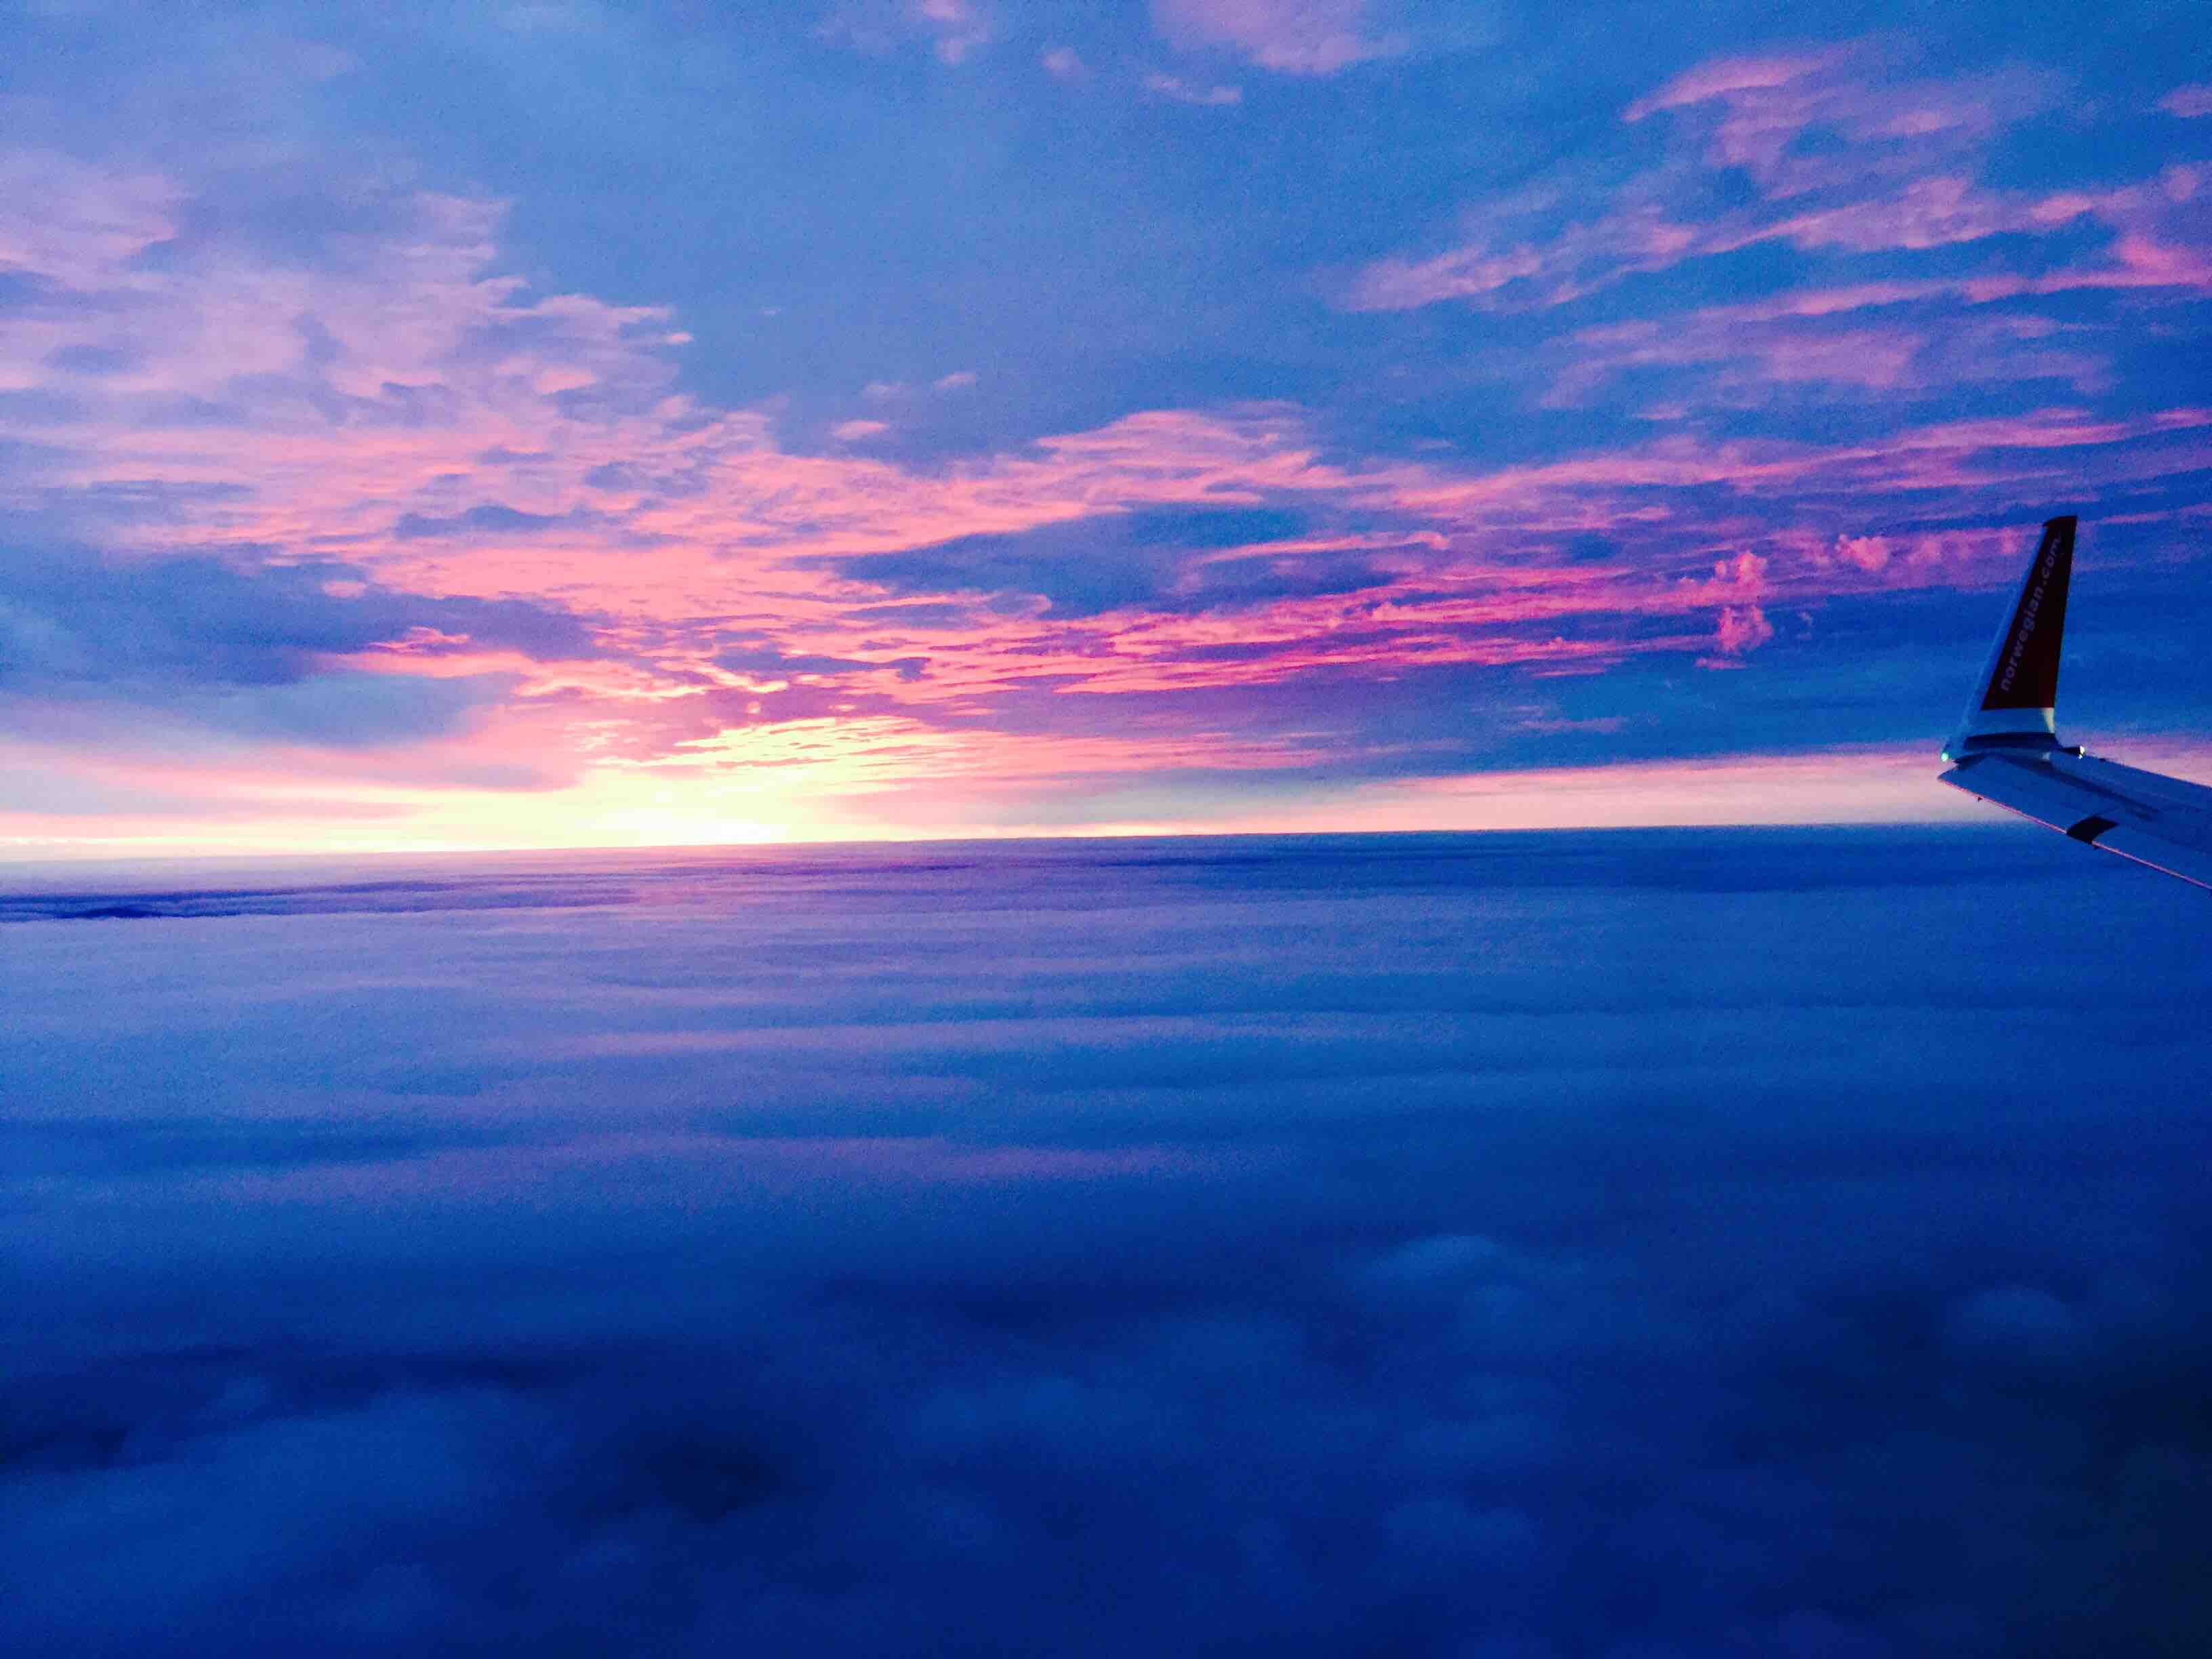
\includegraphics[scale=0.09]{./plots/first.jpg}
		\end{center}
	\end{frame}
	
\aaltotitleframe


\footnotesize


\begin{frame}{}
	\begin{itemize}
		\item Hongyu Su
		\item Born 1984 (integrity, hard-work, open, creative)
		\item I am a postdoc in Helsinki Institute for Information Technology and Aalto University since 2015.5.
		\item Research: build advance machine learning models to solve large scale data analysis problem (research project).
		\item Equivalent to: continuously learning, thinking, implementing, reporting.
	\end{itemize}
	\begin{center}
		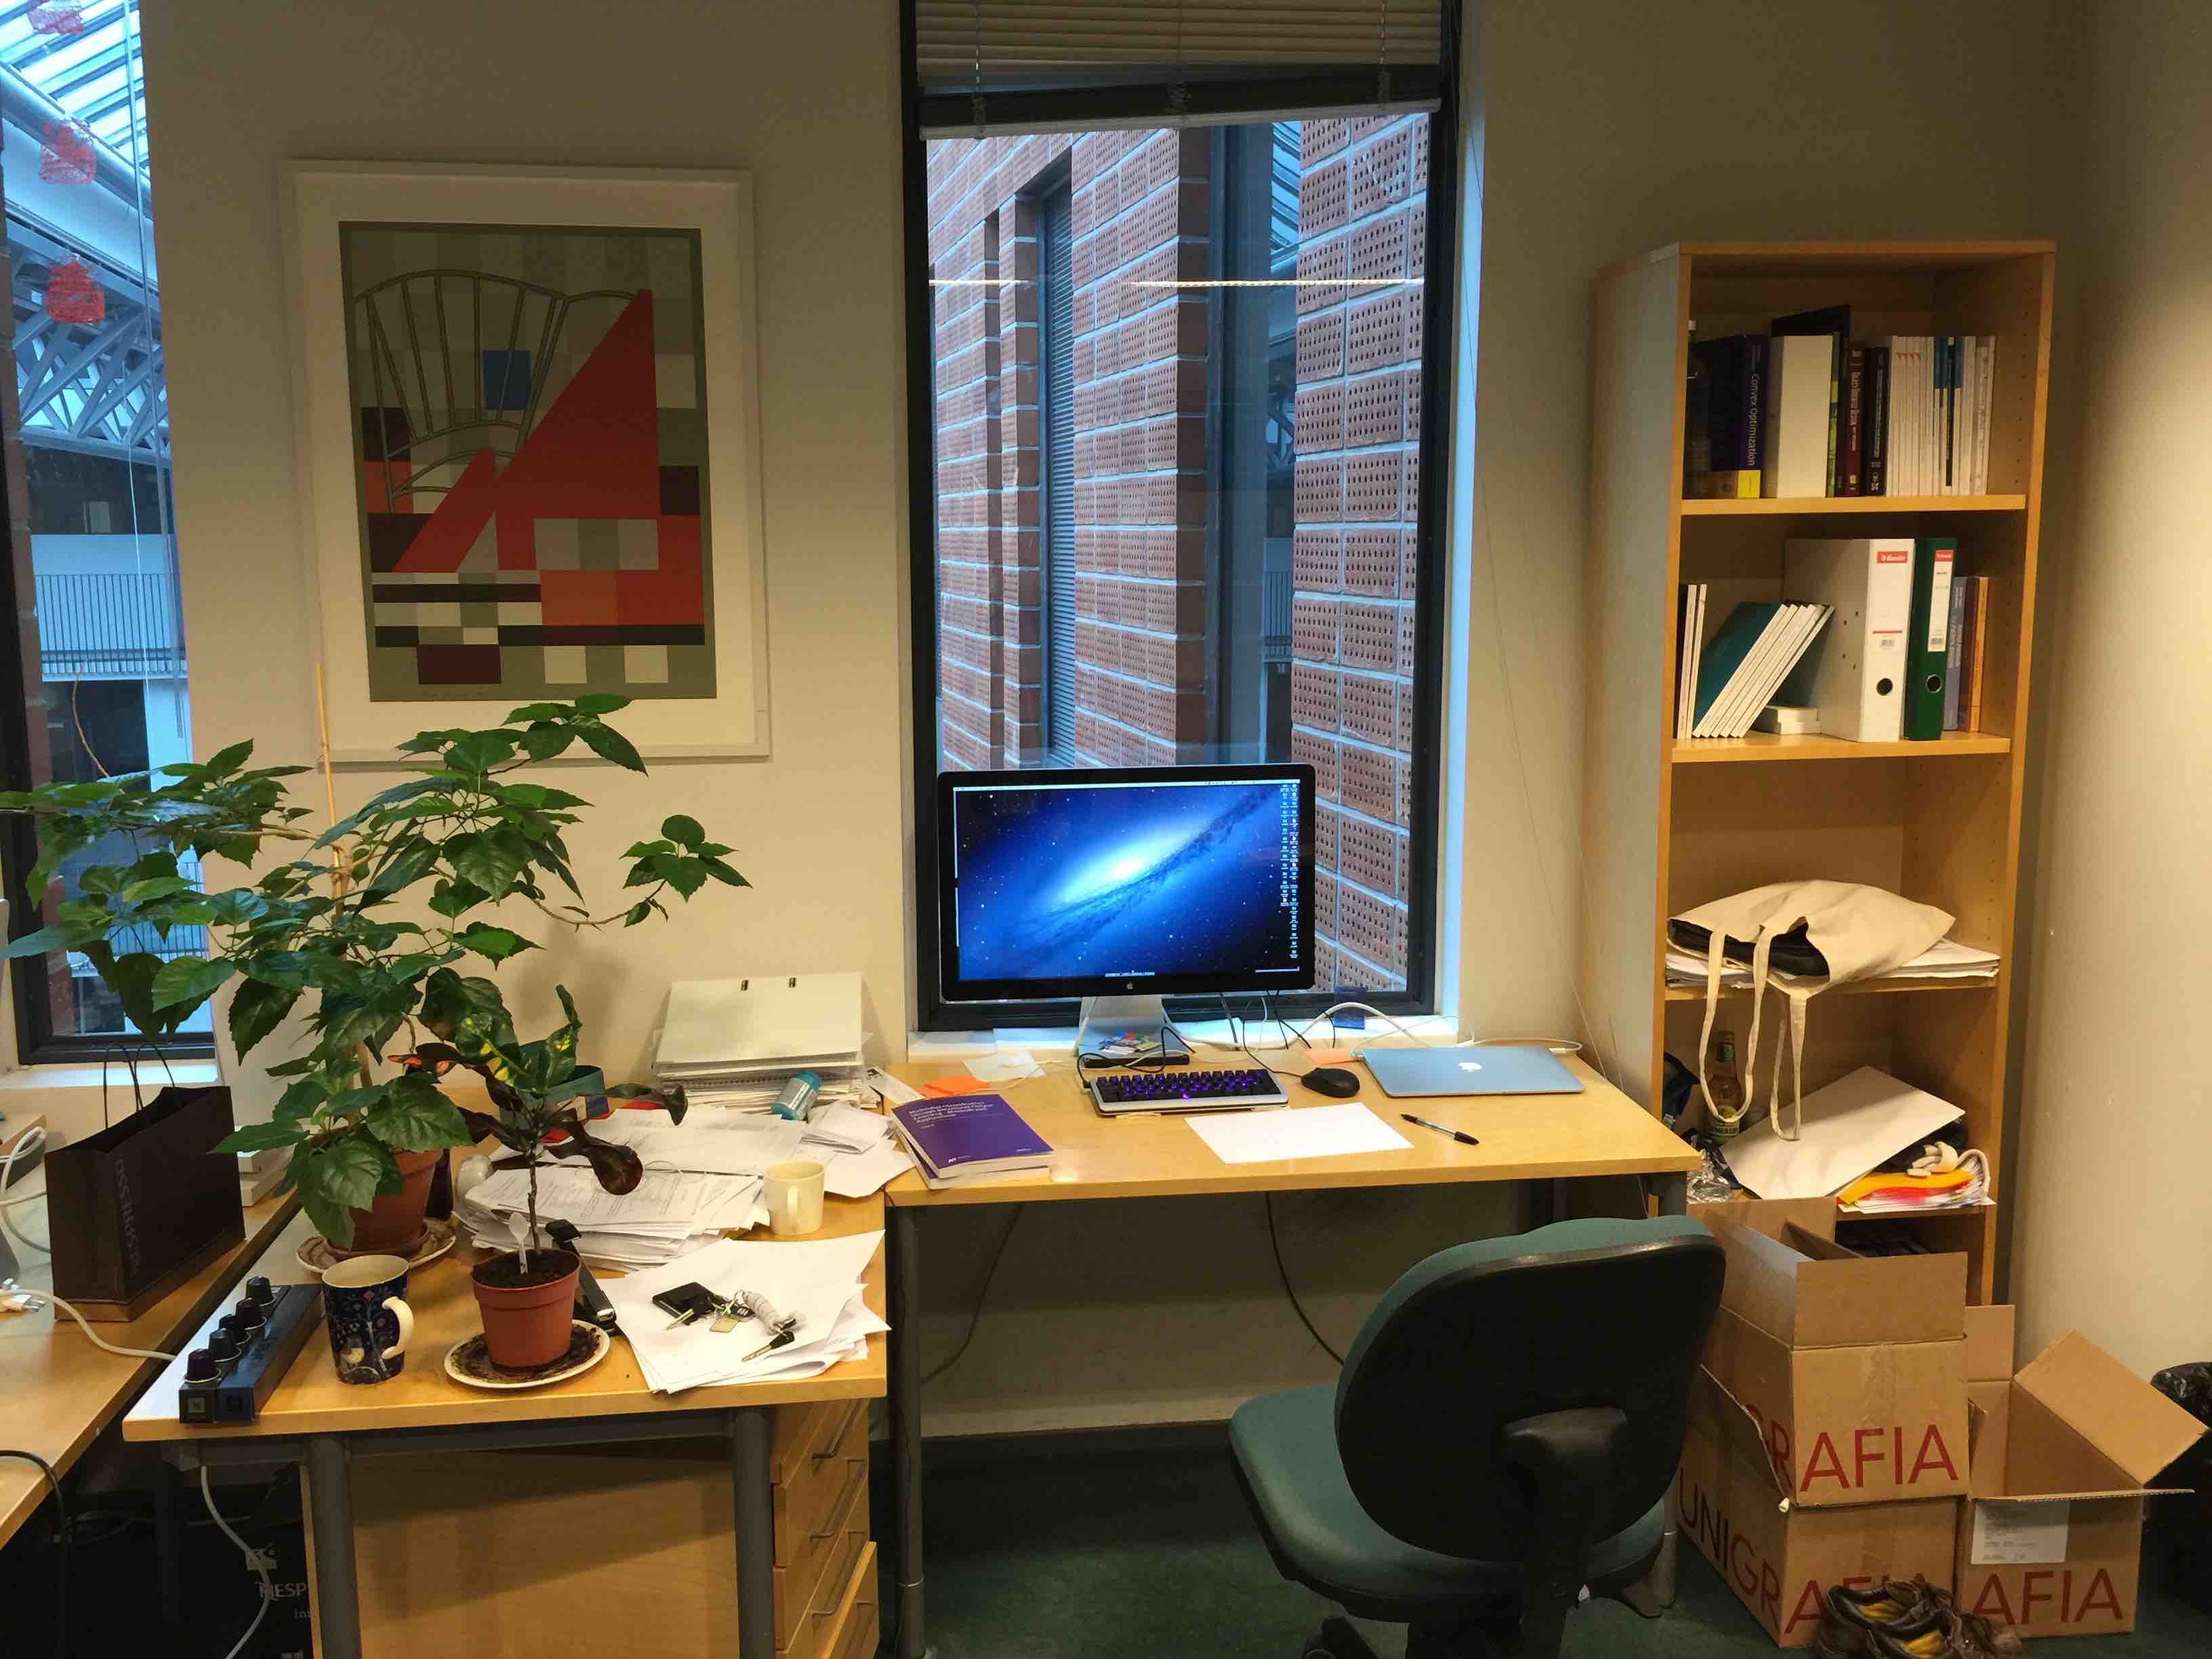
\includegraphics[scale = 0.04]{./plots/office1.jpg}
		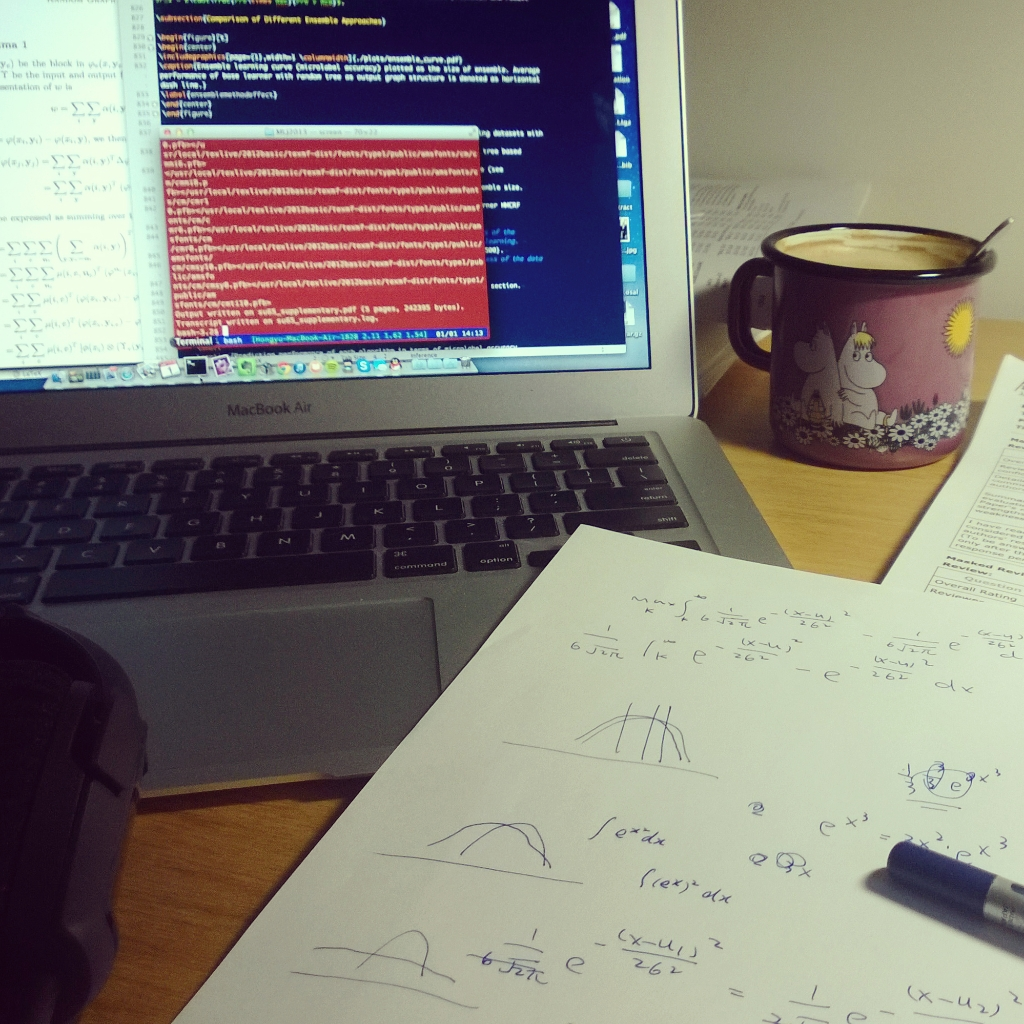
\includegraphics[scale = 0.1]{./plots/office2.jpg}
	\end{center}
\end{frame}

\begin{frame}{Educations}
	\begin{center}
		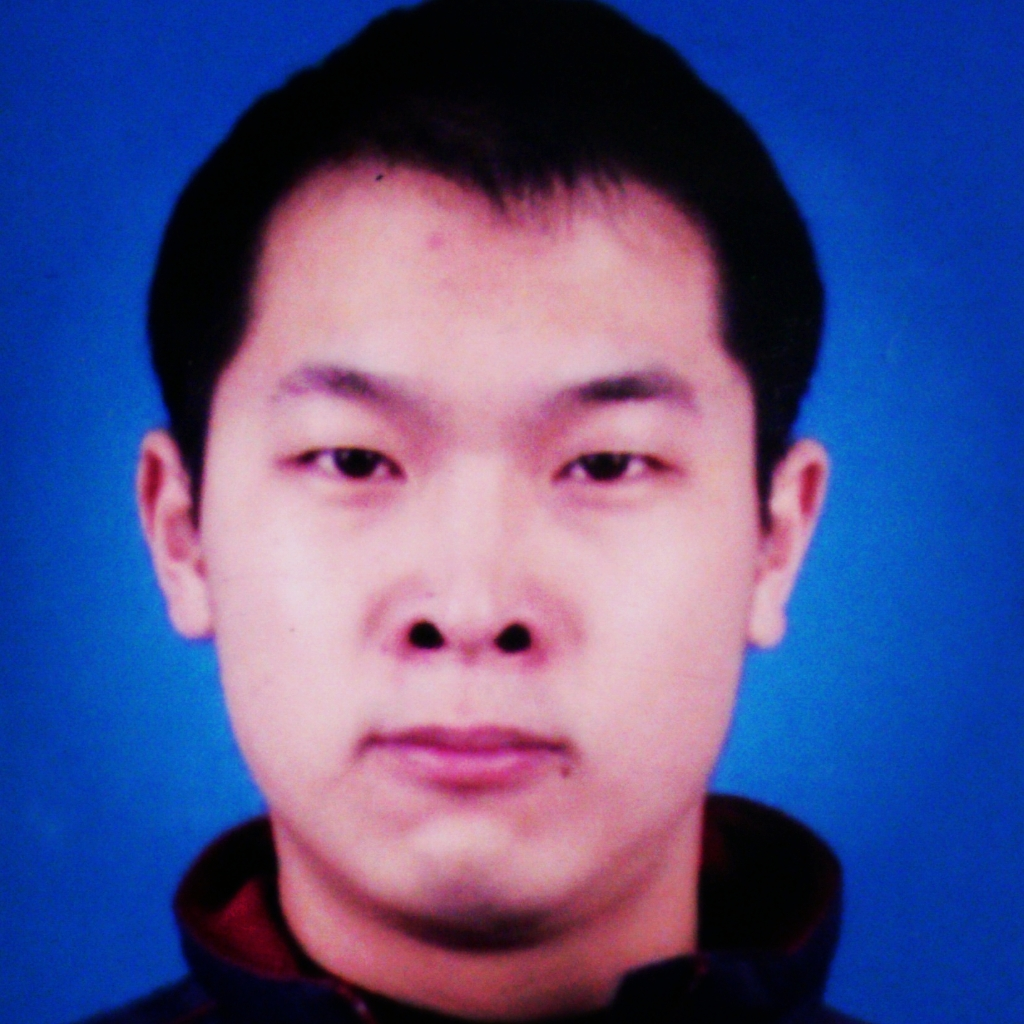
\includegraphics[scale = 0.11]{./plots/photo1.jpg}
		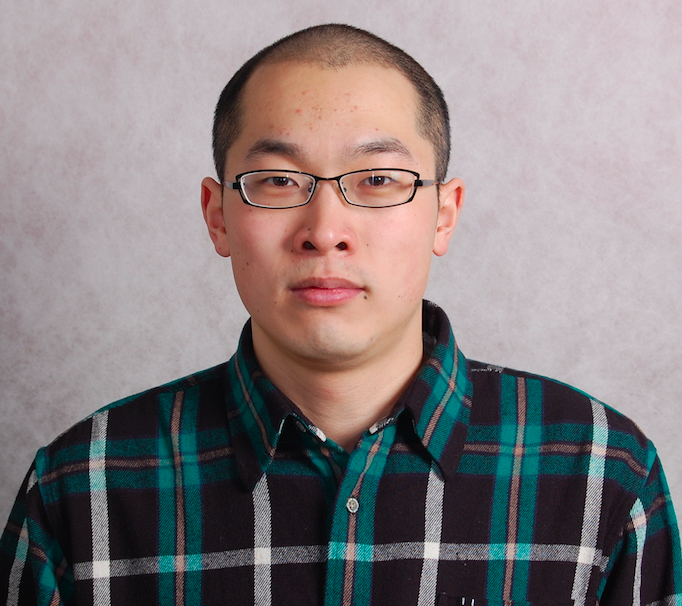
\includegraphics[scale = 0.15]{./plots/photo2.png}
		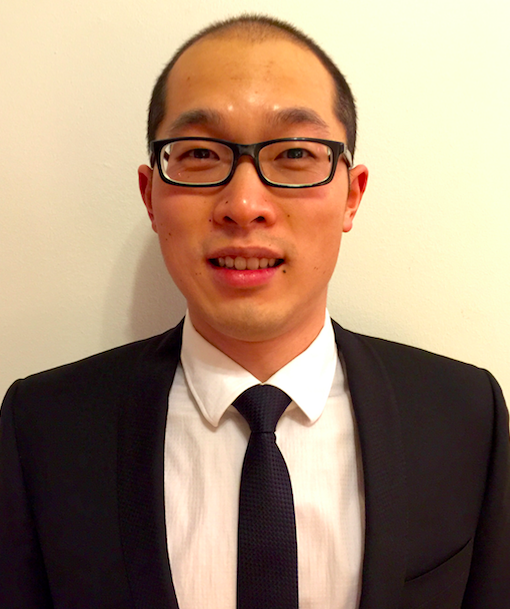
\includegraphics[scale = 0.15]{./plots/photo3.png}
	\end{center}
	\begin{itemize}
		\item Bachelor in Computer Science and Engineering, Xidian University, 2007
		\item Master in Bioinformatics, University of Helsinki, 2010
		\item Phd in Information and Computer Science, Aalto University, 2015
		\item {\em 'Everything comes with a price. Everything. Some things just cost more than others.'} -Brom
		\item Some things don't have a price tag!
	\end{itemize}
\end{frame}

\begin{frame}{Phd, 2011.01-2015.04, Helsinki, Finland}
	\begin{itemize}
		\item The topic is {\bf machine learning and optimization research on structured data}.
		\item Machine learning is to estimate outcomes (unknown) from data (known).
		\item {\bf Ask non-trivial machine learning questions and provide solutions.}
		\begin{itemize}\footnotesize
			\item Computer vision, identify object in the image.
			\begin{tabular}{p{3cm}p{10cm}}
	        \multirow{2}{*}{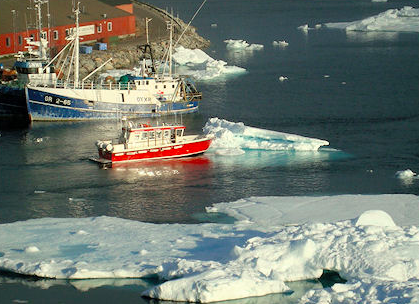
\includegraphics[scale = 0.13]{./plots/boatsea.png}} & \\
			& $(\underbrace{+1}_{\text{boat}},\underbrace{+1}_{\text{sea}},\underbrace{-1}_{\text{sun}},\underbrace{-1}_{\text{beach}},\underbrace{-1}_{\text{people}},\underbrace{+1}_{\text{ice}},\underbrace{+1}_{\text{land}})$\\
	        \end{tabular}
	\vspace{0.3cm}
			\item News articles can be assigned to multiple categories.
			\begin{tabular}{p{3cm}p{10cm}} 
	        \multirow{2}{*}{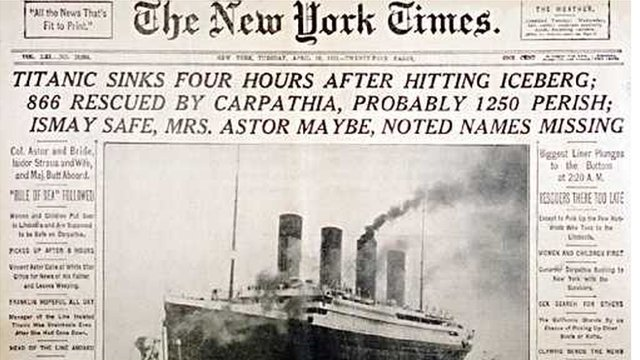
\includegraphics[scale = 0.13]{./plots/titanic.jpg}} & \\
			& $(\underbrace{+1}_{\text{news}},\underbrace{+1}_{\text{economics}},\underbrace{-1}_{\text{sports}},\underbrace{-1}_{\text{politics}},\underbrace{-1}_{\text{movie}},\underbrace{-1}_{\text{science}},\underbrace{-1}_{\text{art}})$\\
	        \end{tabular}
		\end{itemize}
	\end{itemize}
\end{frame}

\begin{frame}{Results}
	Methods and technologies that are published in {\bf TOP} machine learning journal and conference.
	\begin{center}
		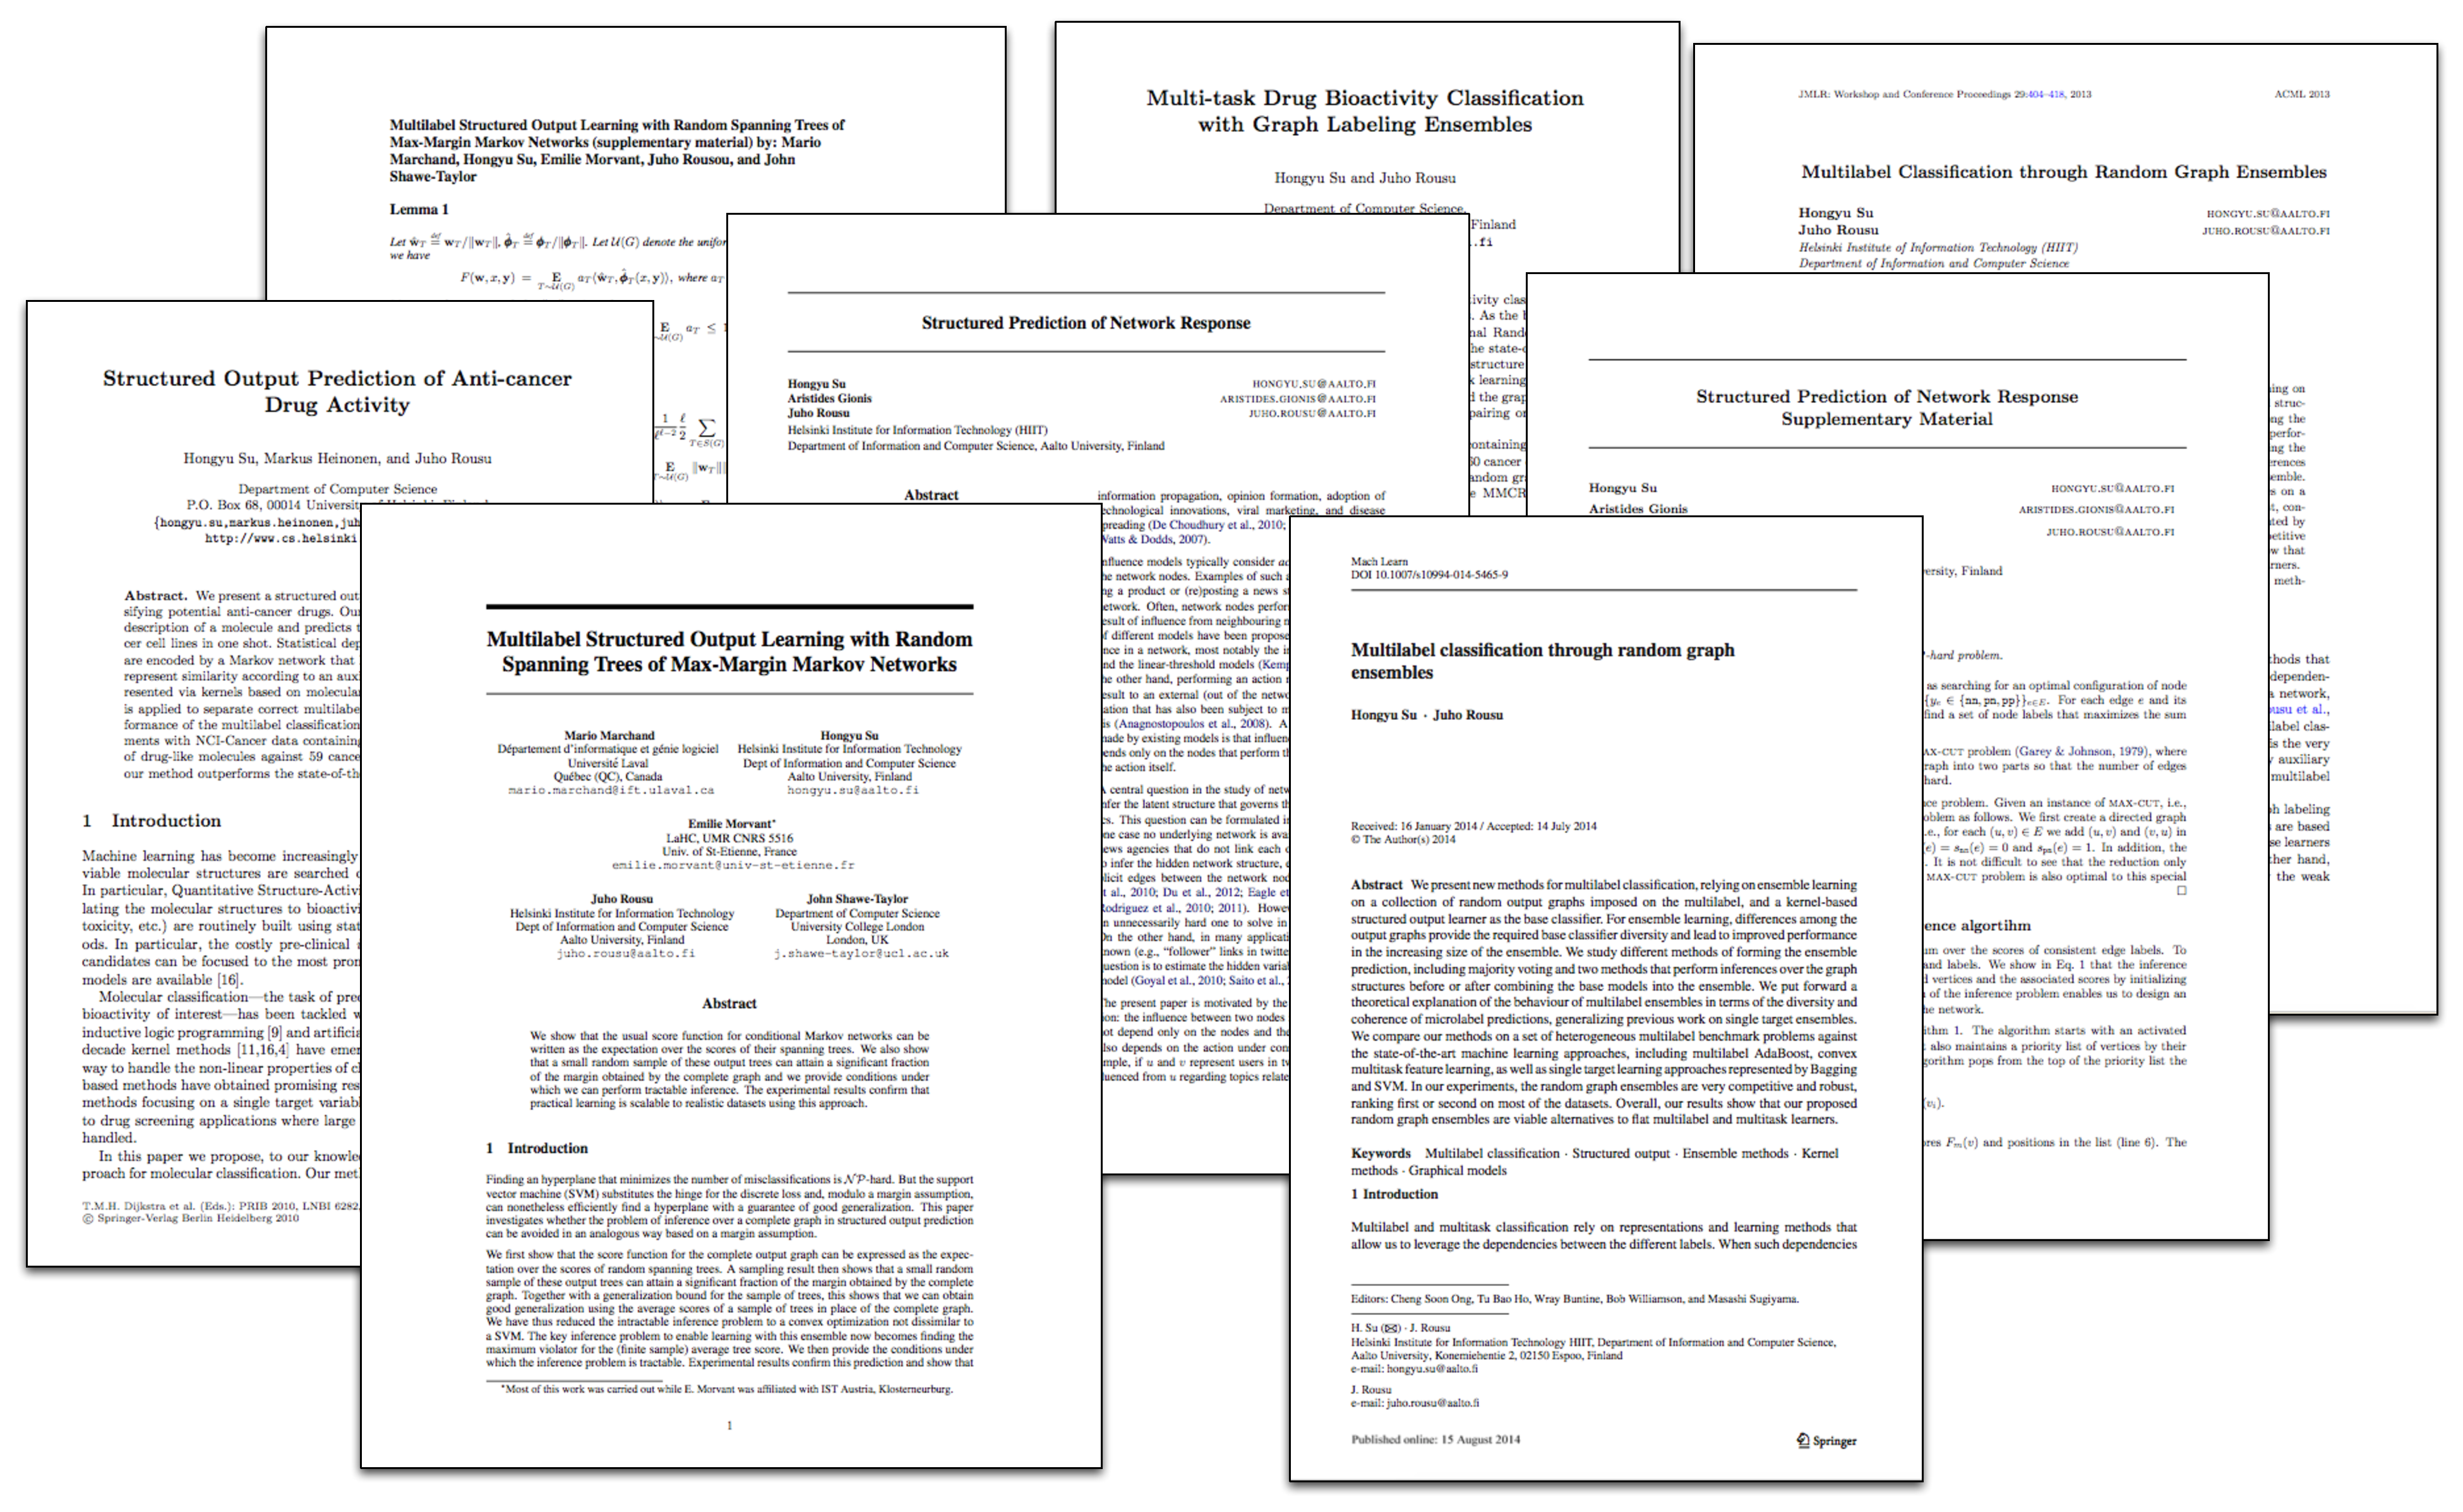
\includegraphics[scale=0.15]{./plots/paperCollection.pdf}
	\end{center}
\end{frame}

\begin{frame}{Dissertation}
	\begin{itemize}
		\item My dissertation {\bf Multilabel classification through structured output learning - methods and applications}.
		\begin{itemize}\footnotesize
			\item {\bf Advanced} machine learning methods to push the boundary of multilabel classification.
			\item Solving many real-world {\bf nontrivial} machine learning problems: document classification, image annotations, molecular classification, bioinformatics, social network analysis.
		\end{itemize}
		\begin{center}
			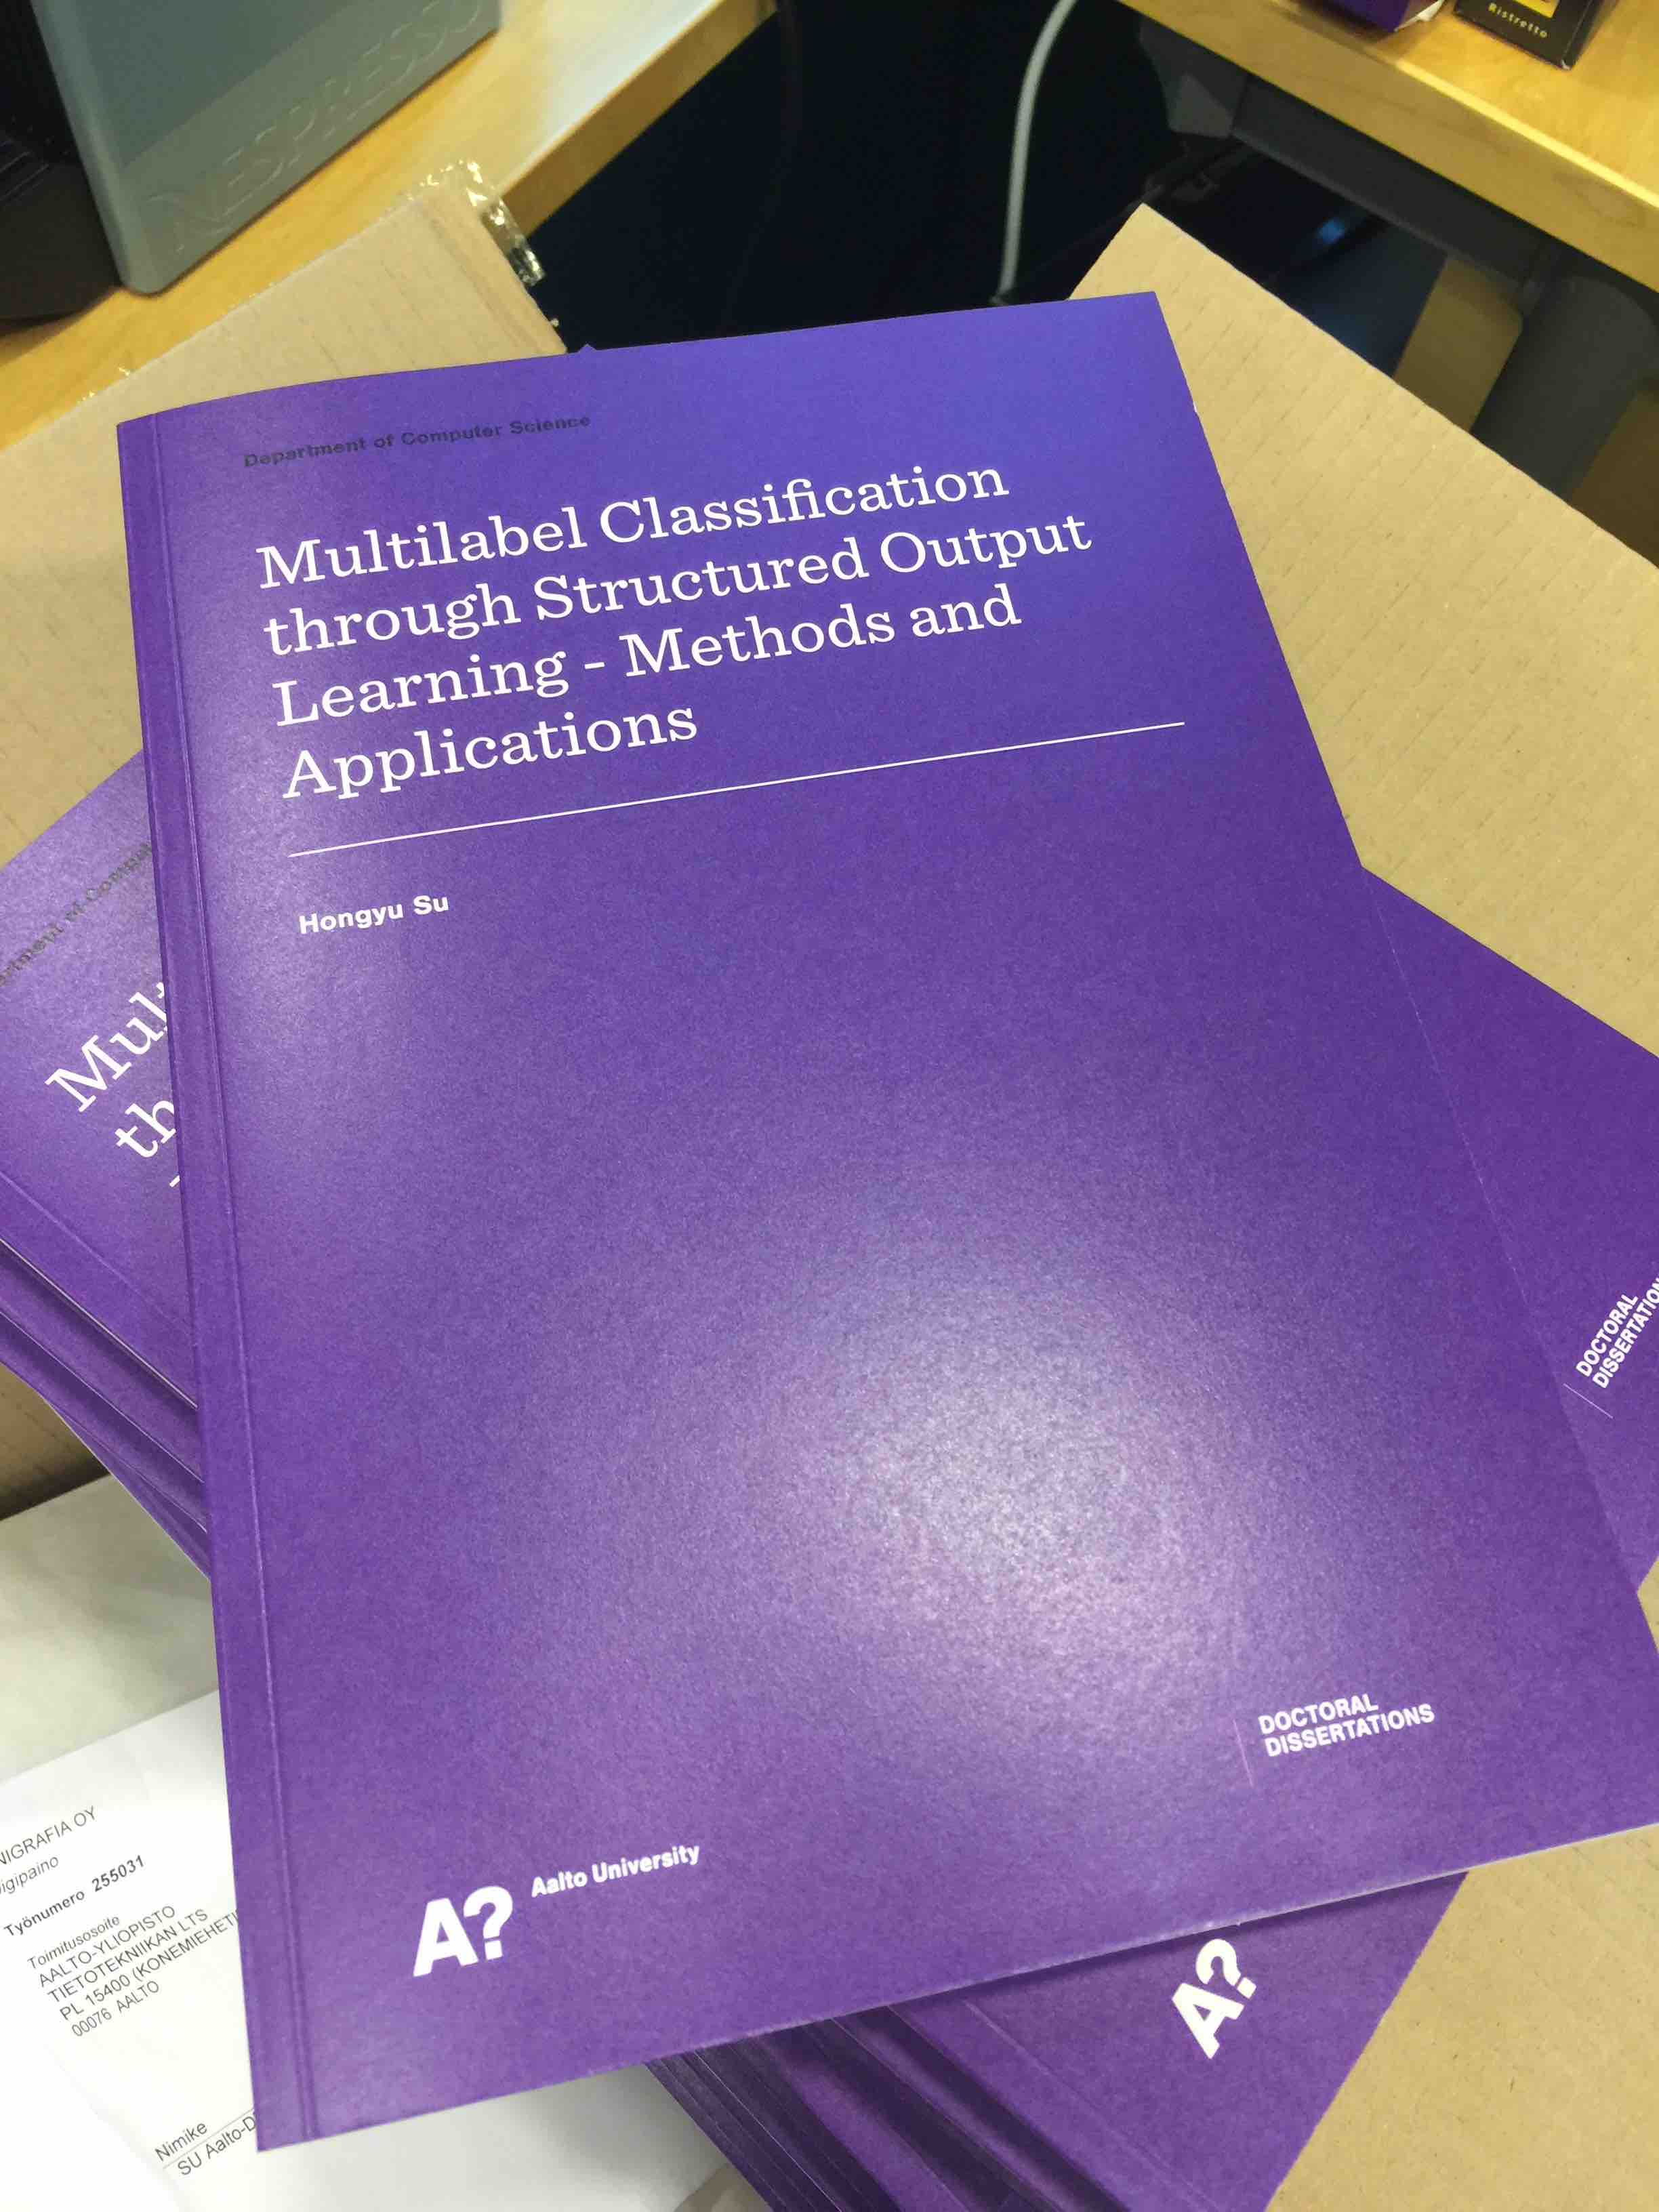
\includegraphics[scale=0.03,angle=-90]{./plots/book.jpg}
		\end{center}
	\end{itemize}
\end{frame}

\begin{frame}{Work hard for 4 years and then}
	\begin{itemize}
		\item Defense
		\begin{center}
			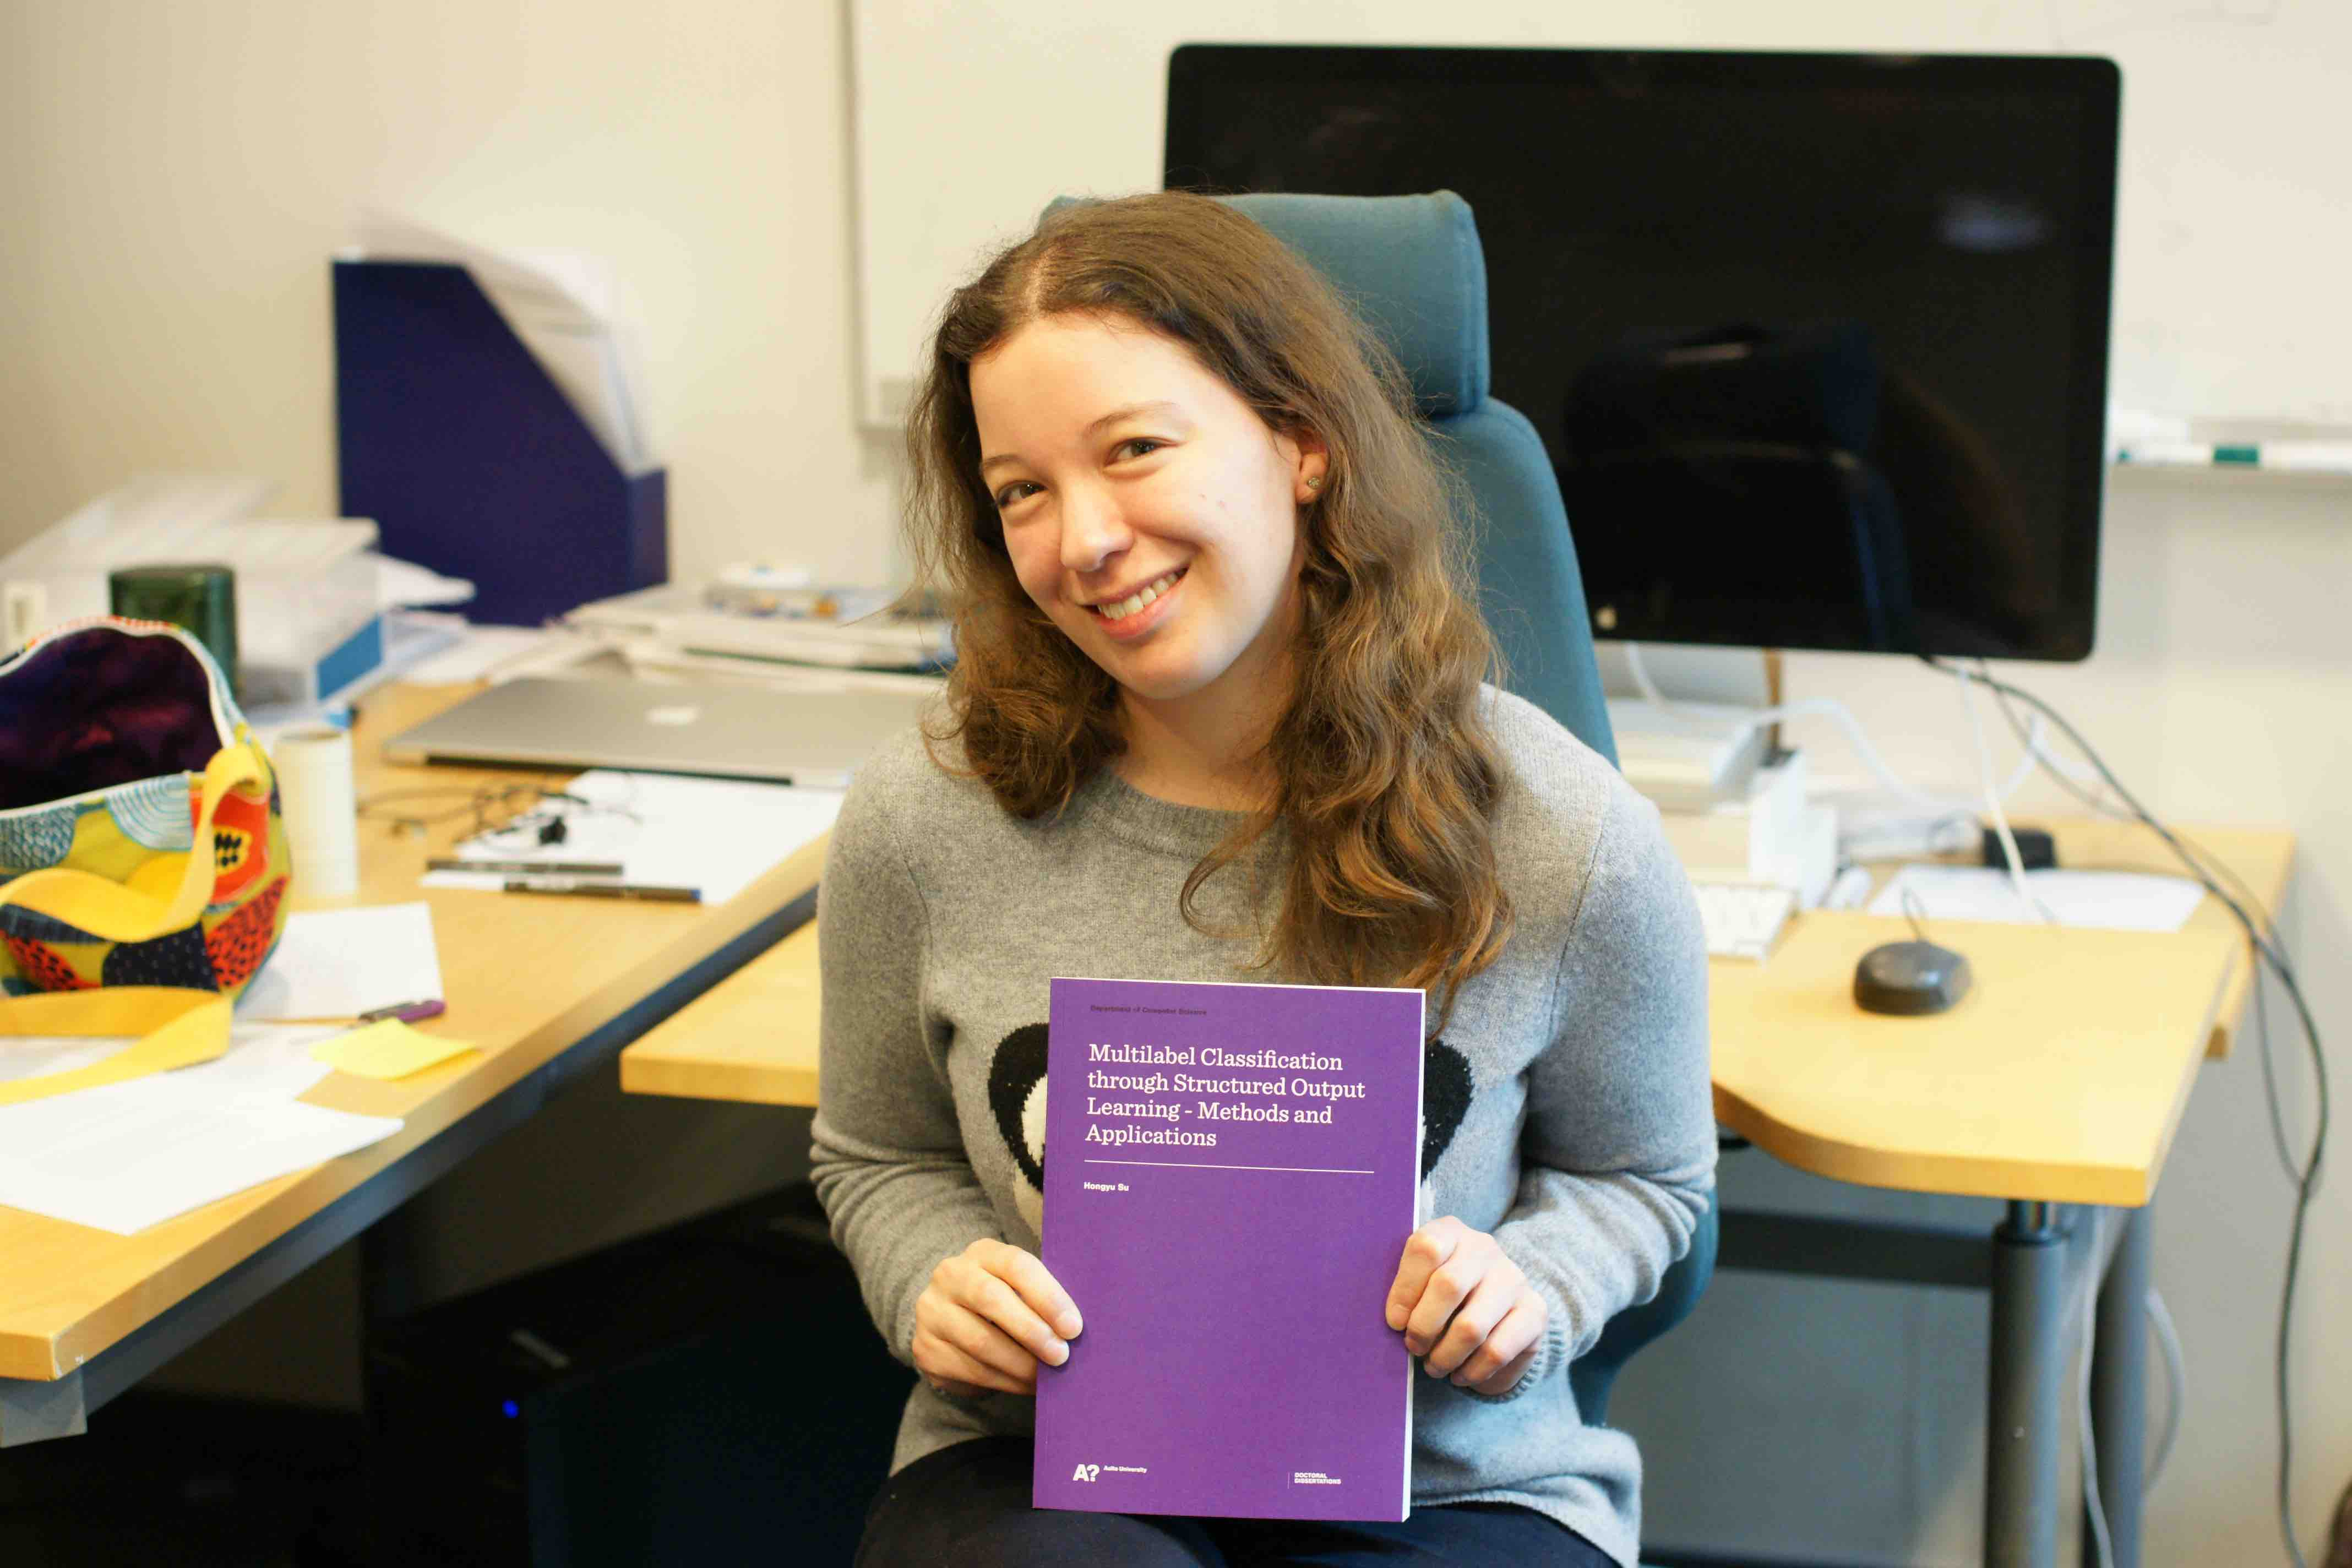
\includegraphics[scale=0.02,angle=0]{./plots/df2.jpg}
			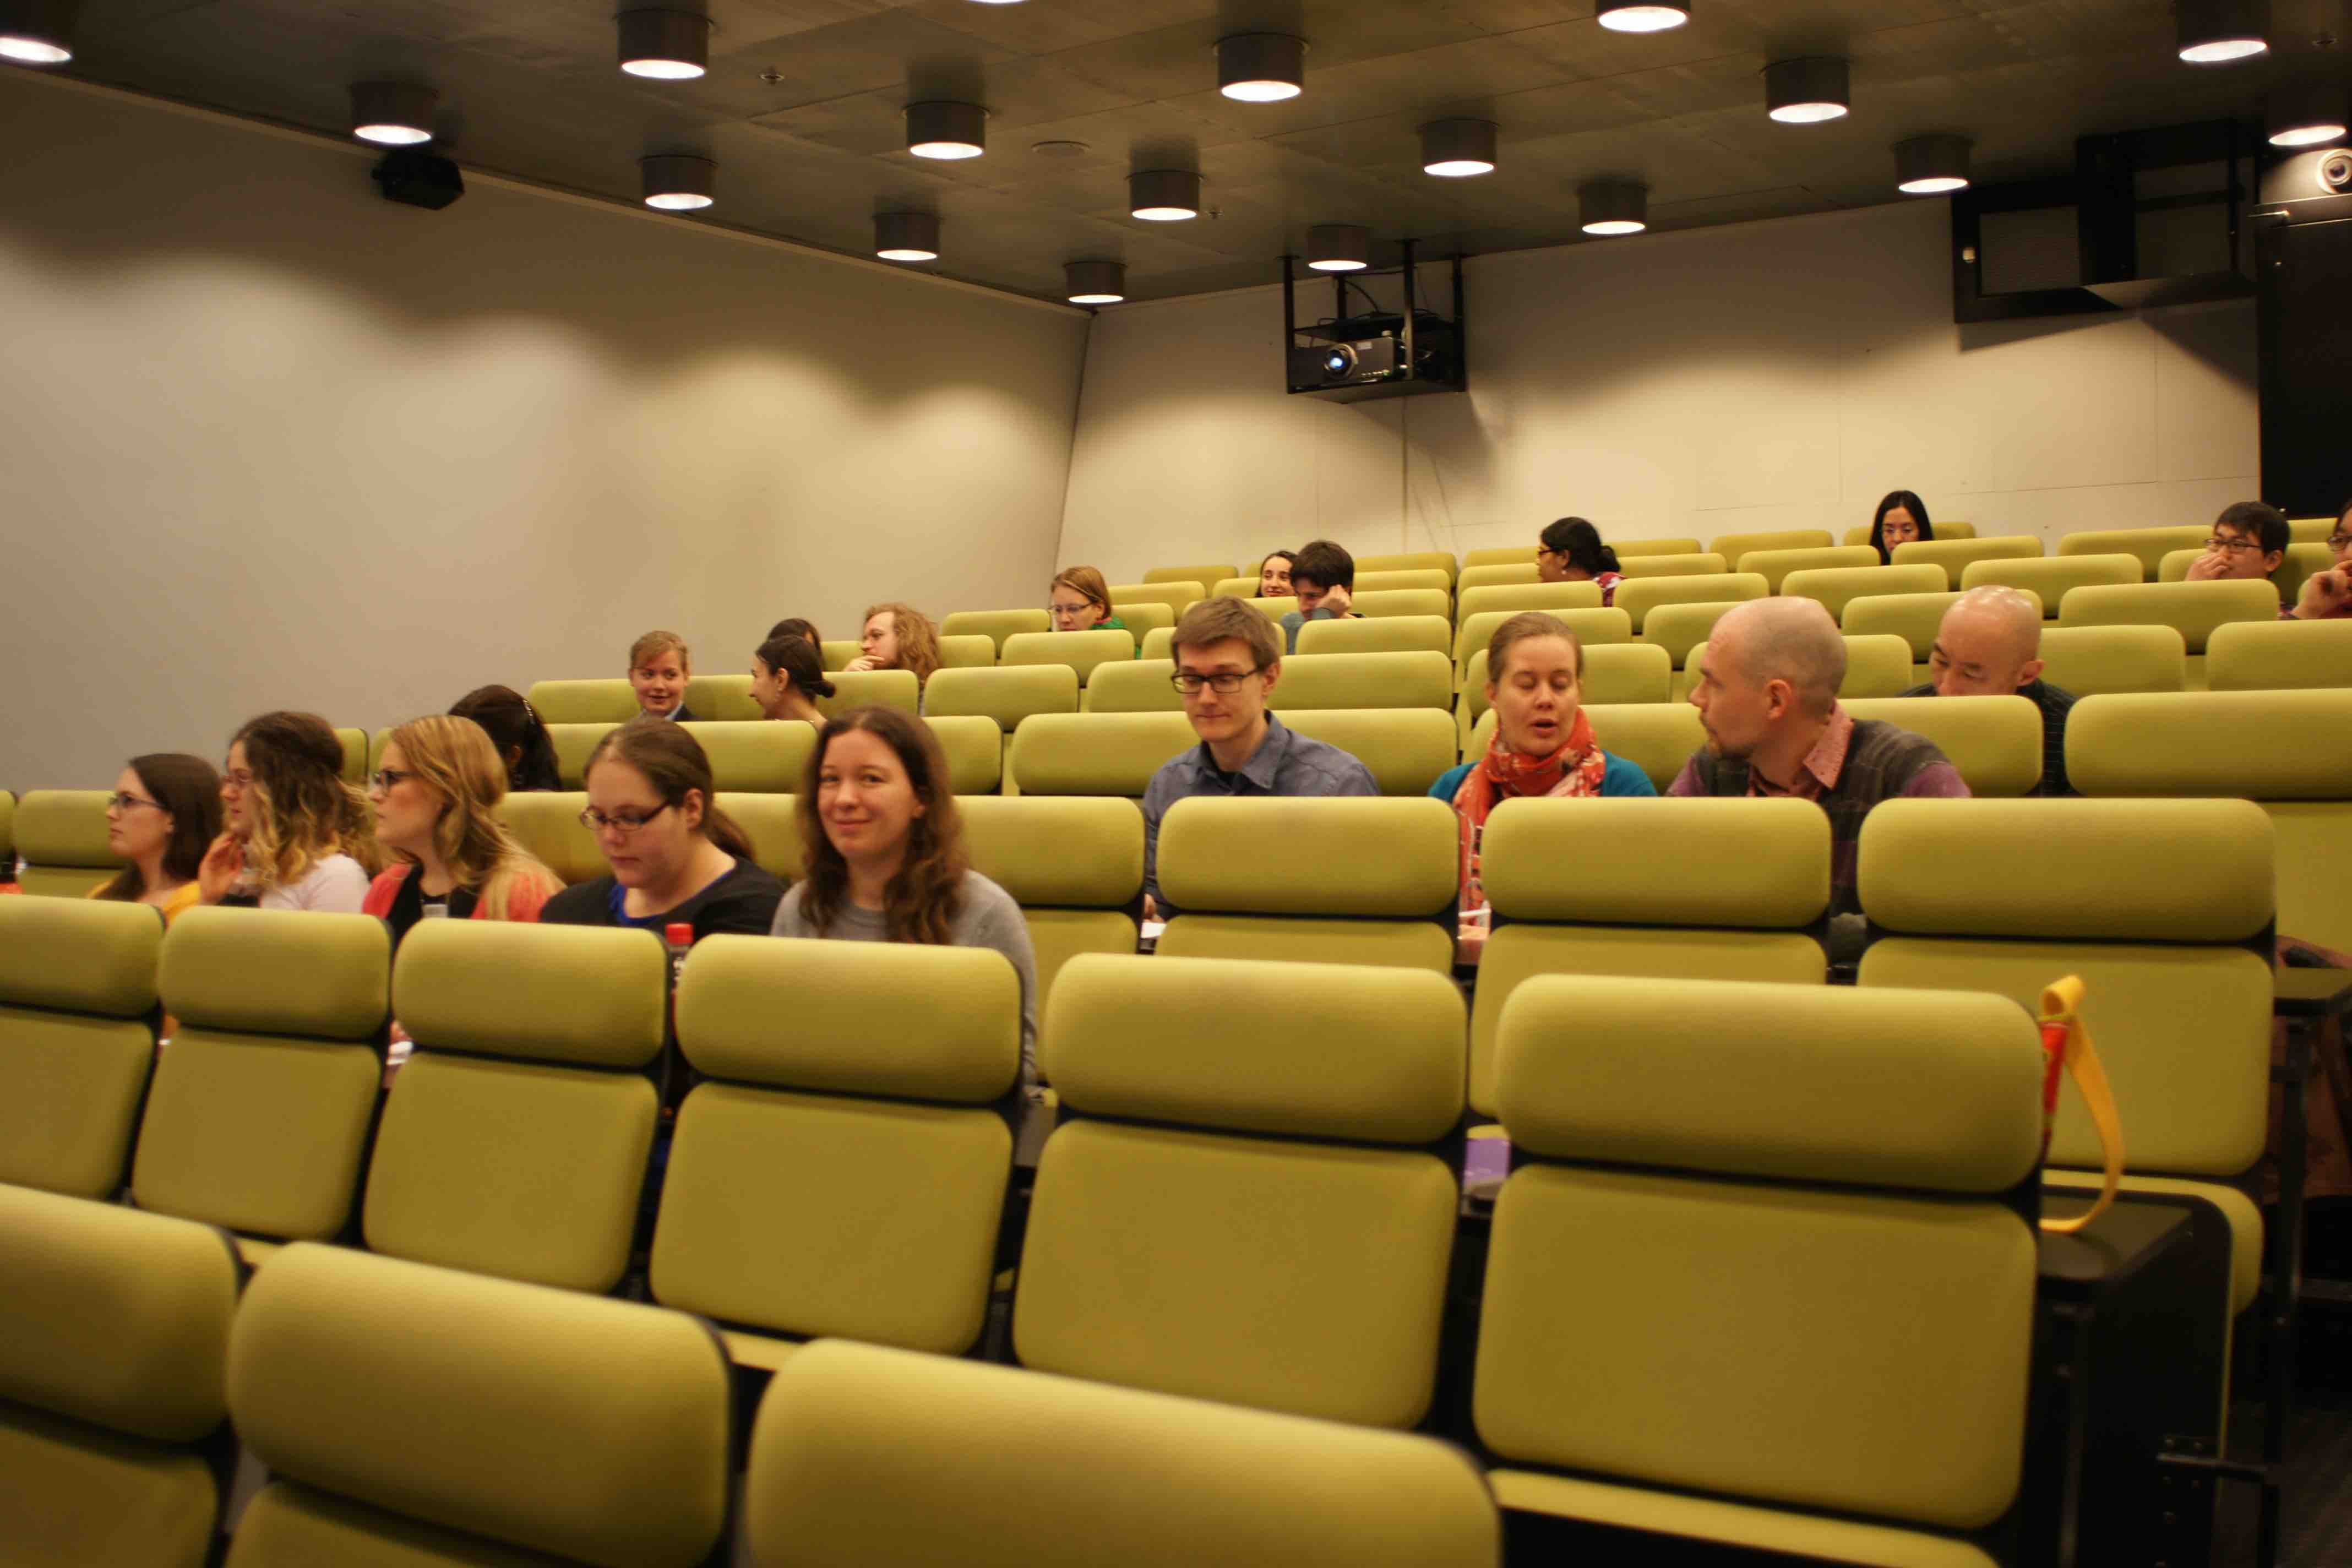
\includegraphics[scale=0.02,angle=0]{./plots/df3.jpg}
			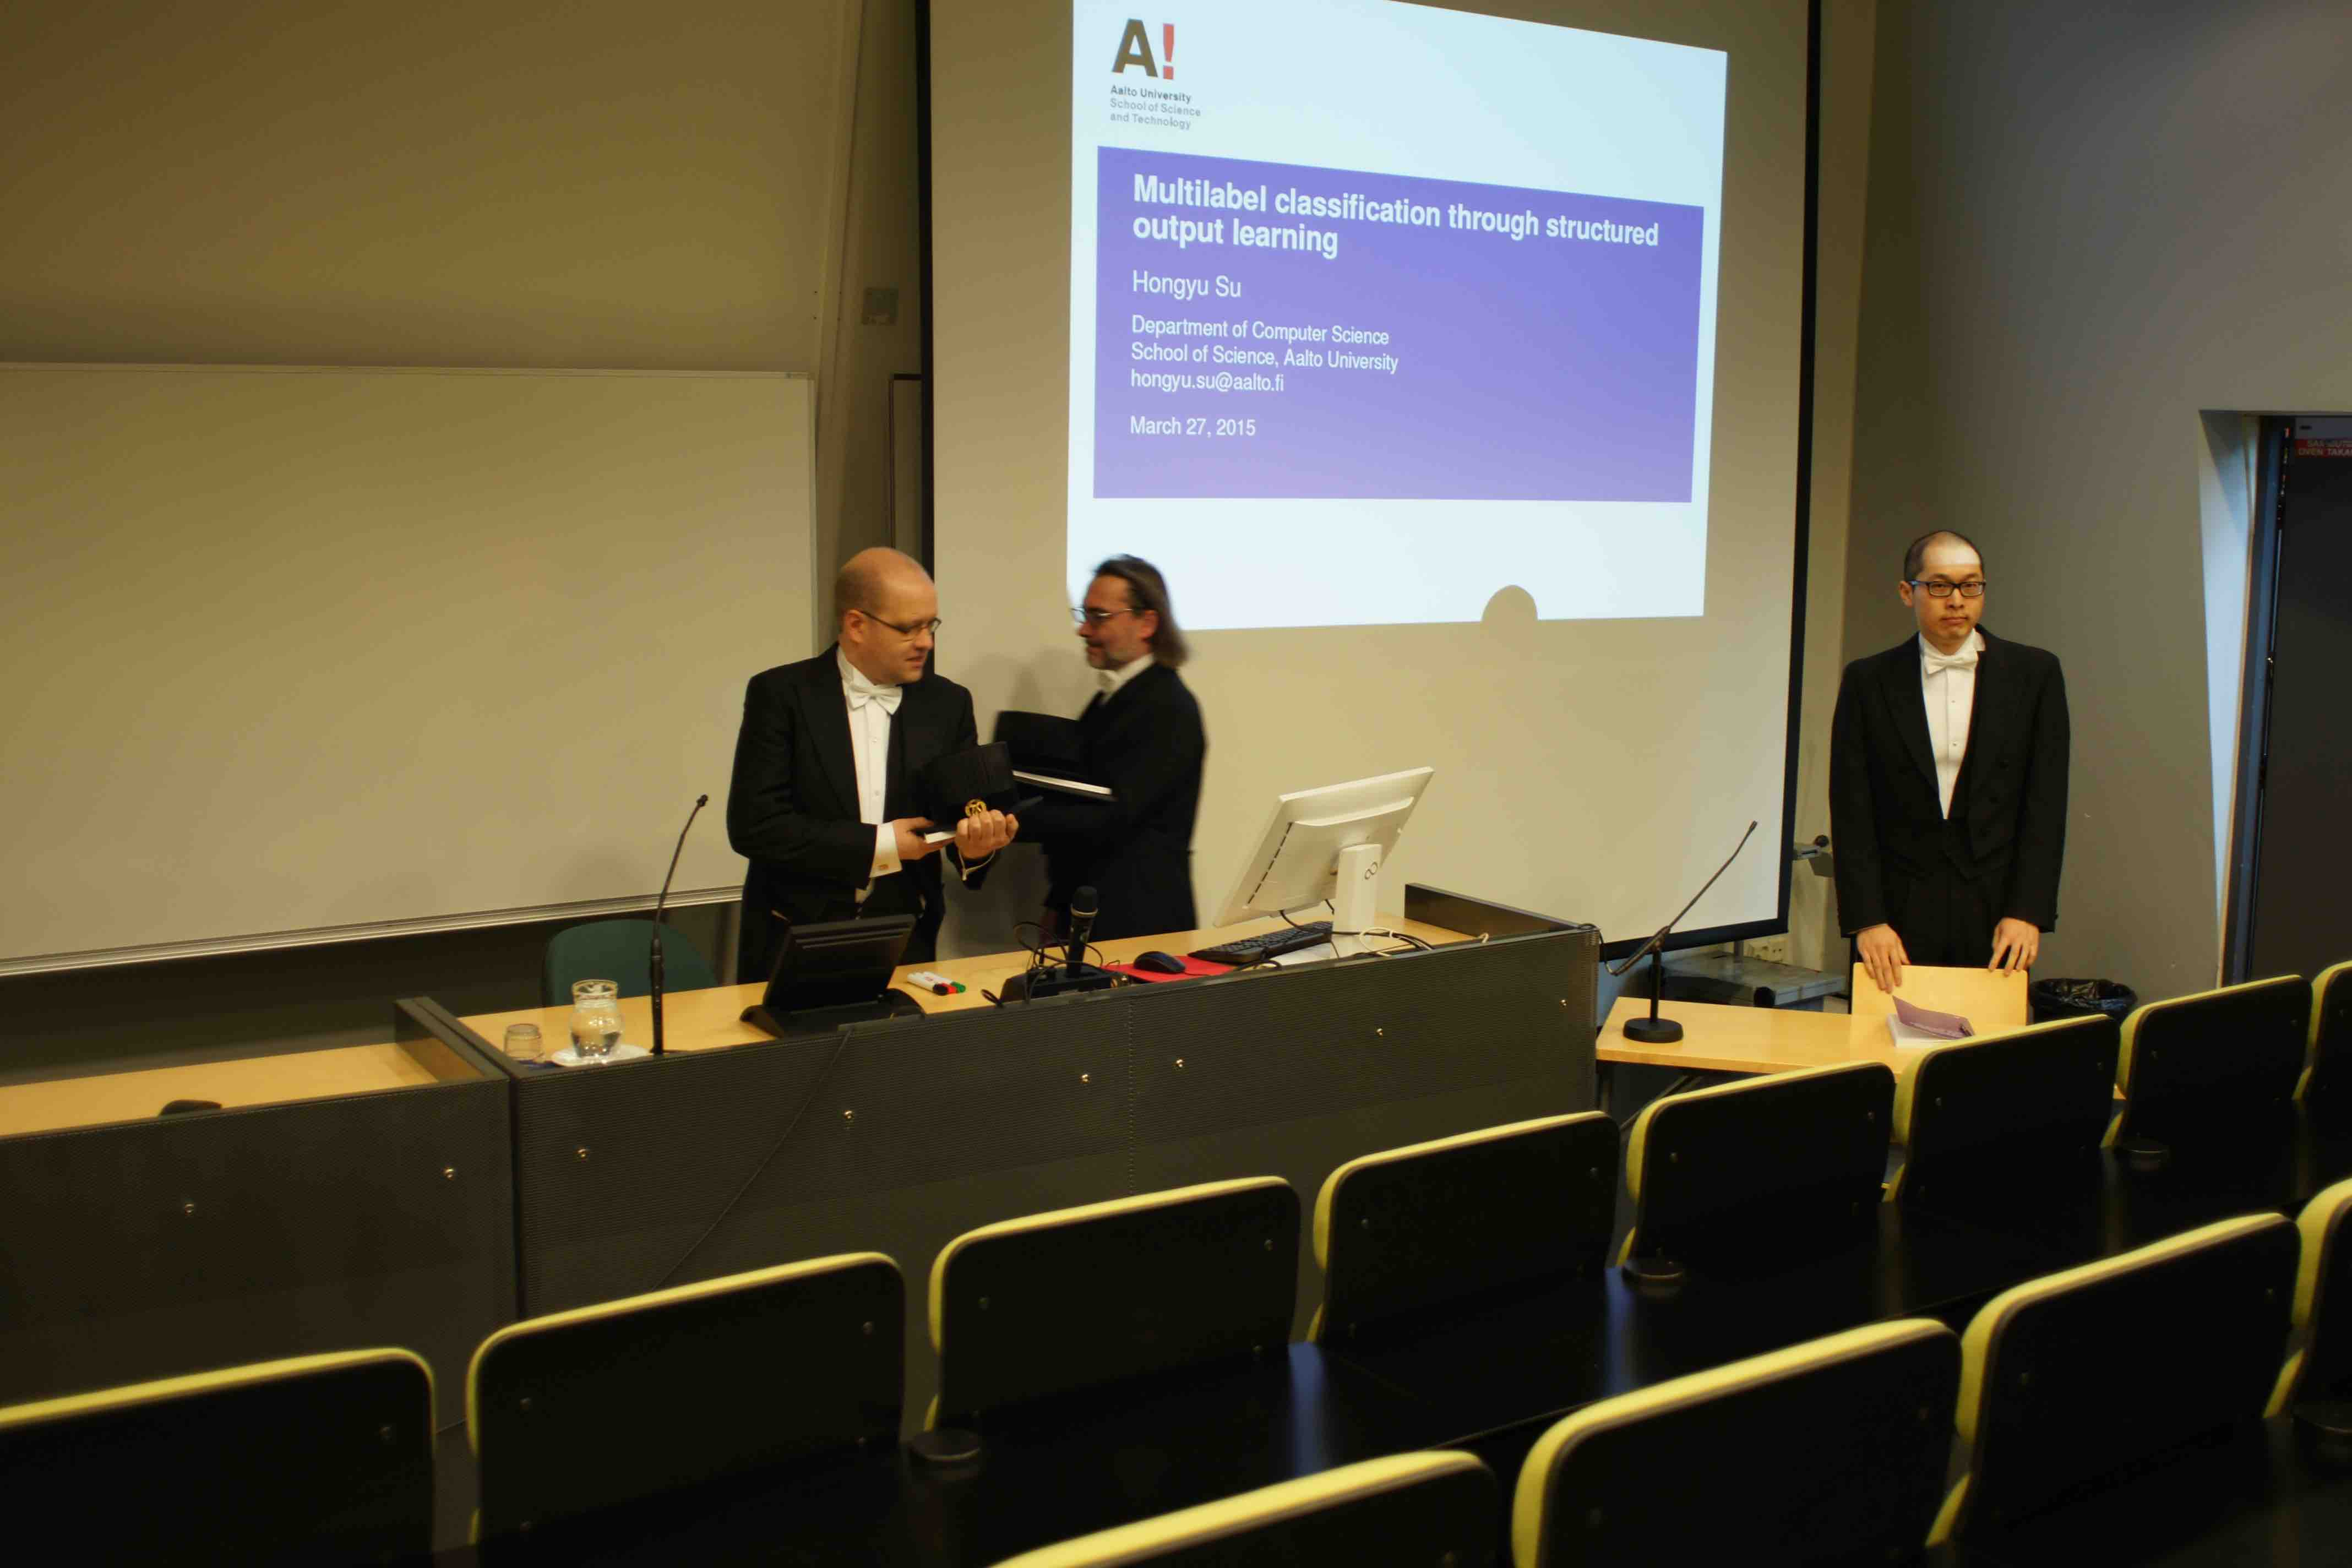
\includegraphics[scale=0.02,angle=0]{./plots/df4.jpg}
		\end{center}
		\item Karonkka
		\begin{center}
			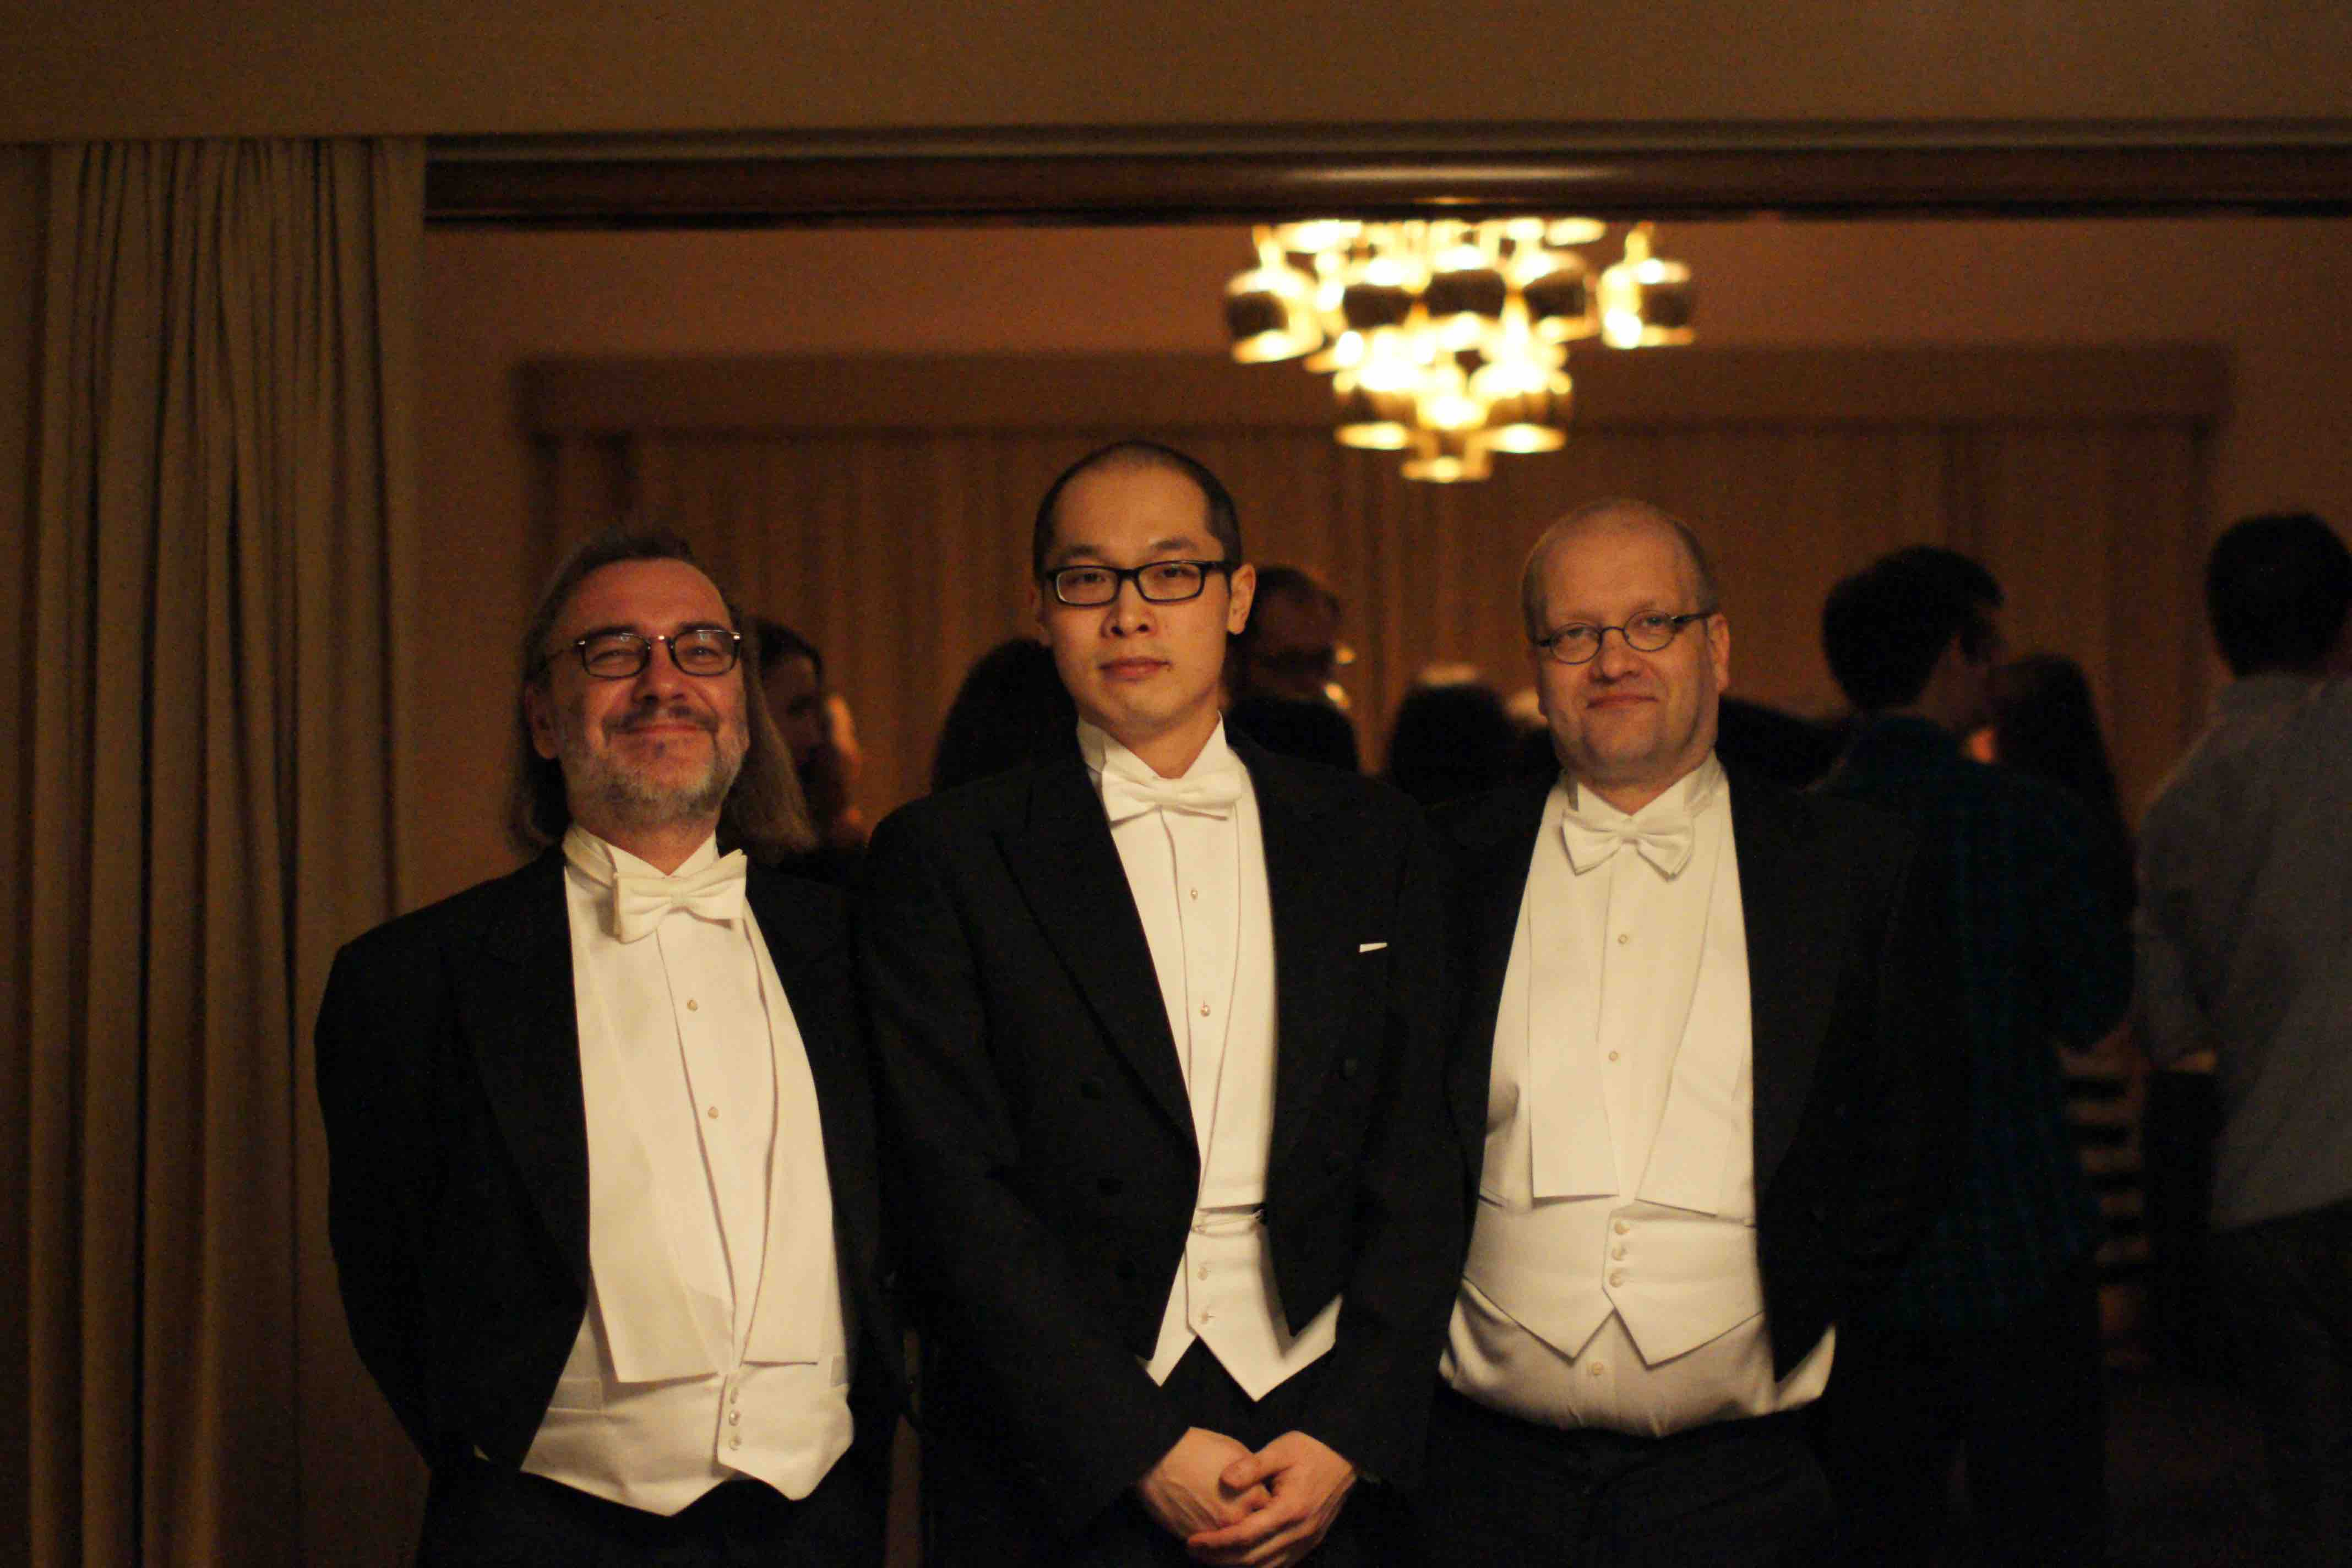
\includegraphics[scale=0.02,angle=0]{./plots/kk1.jpg}			
			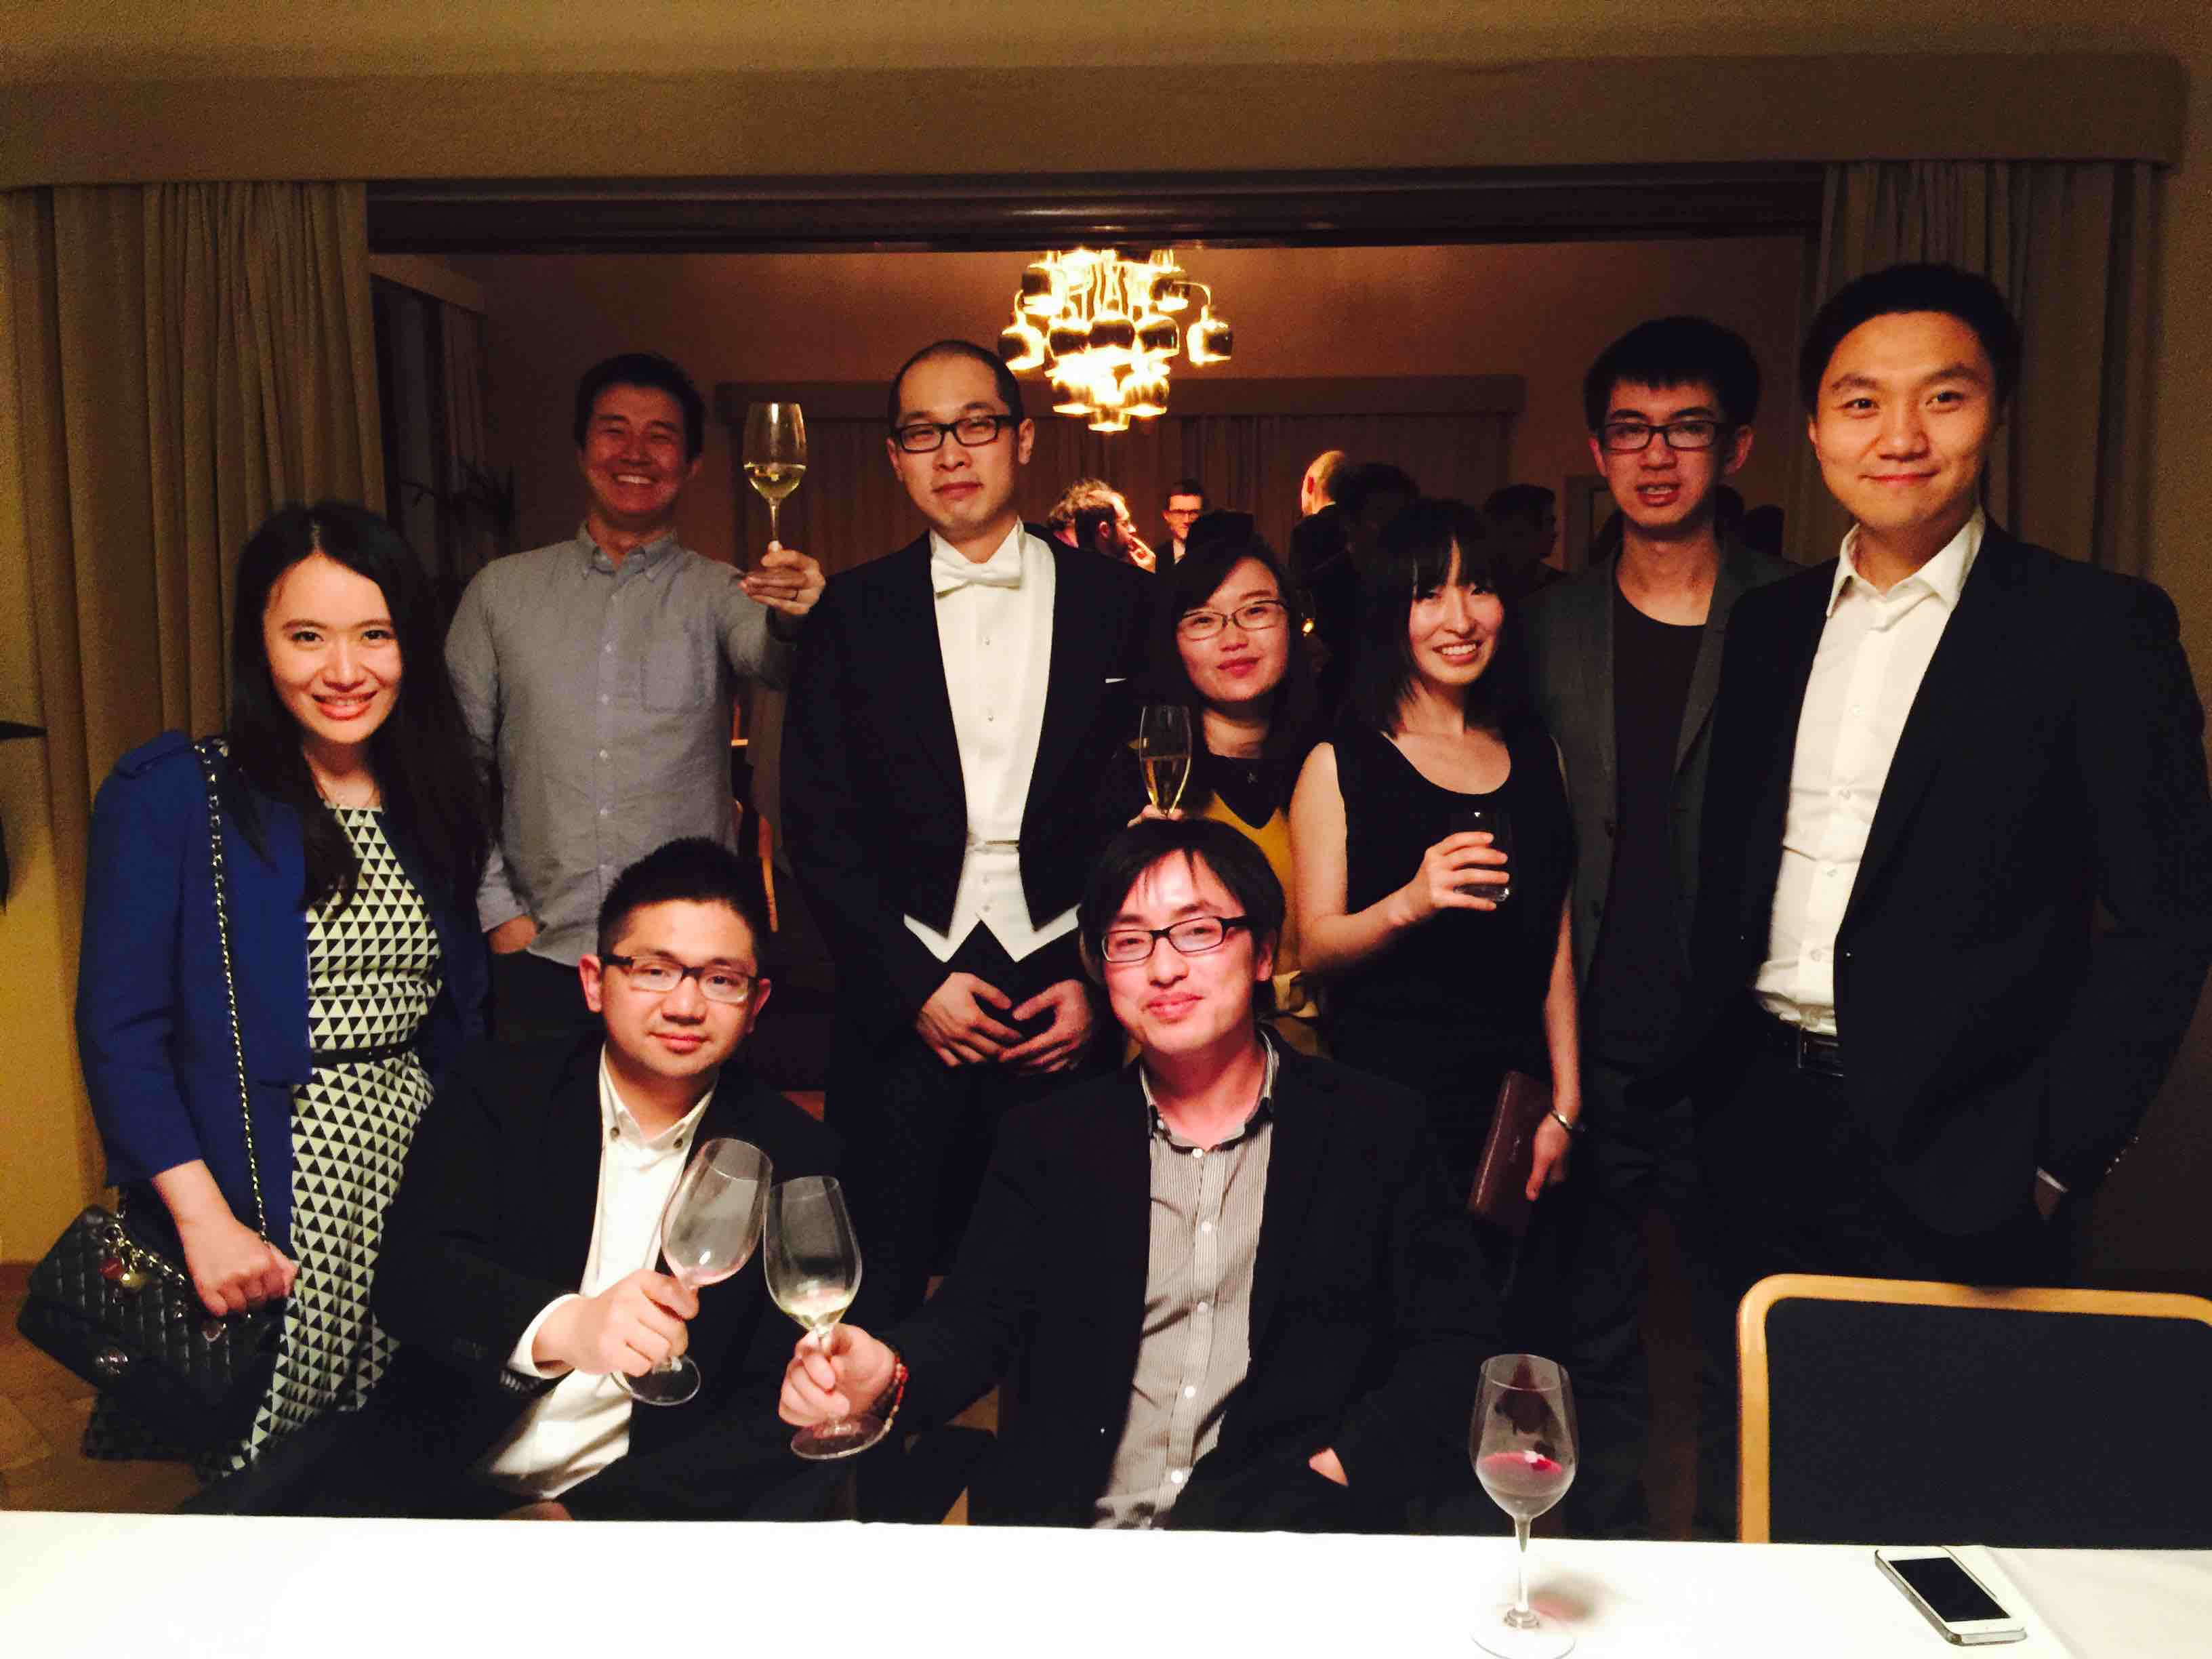
\includegraphics[scale=0.023,angle=0]{./plots/kk2.jpg}
			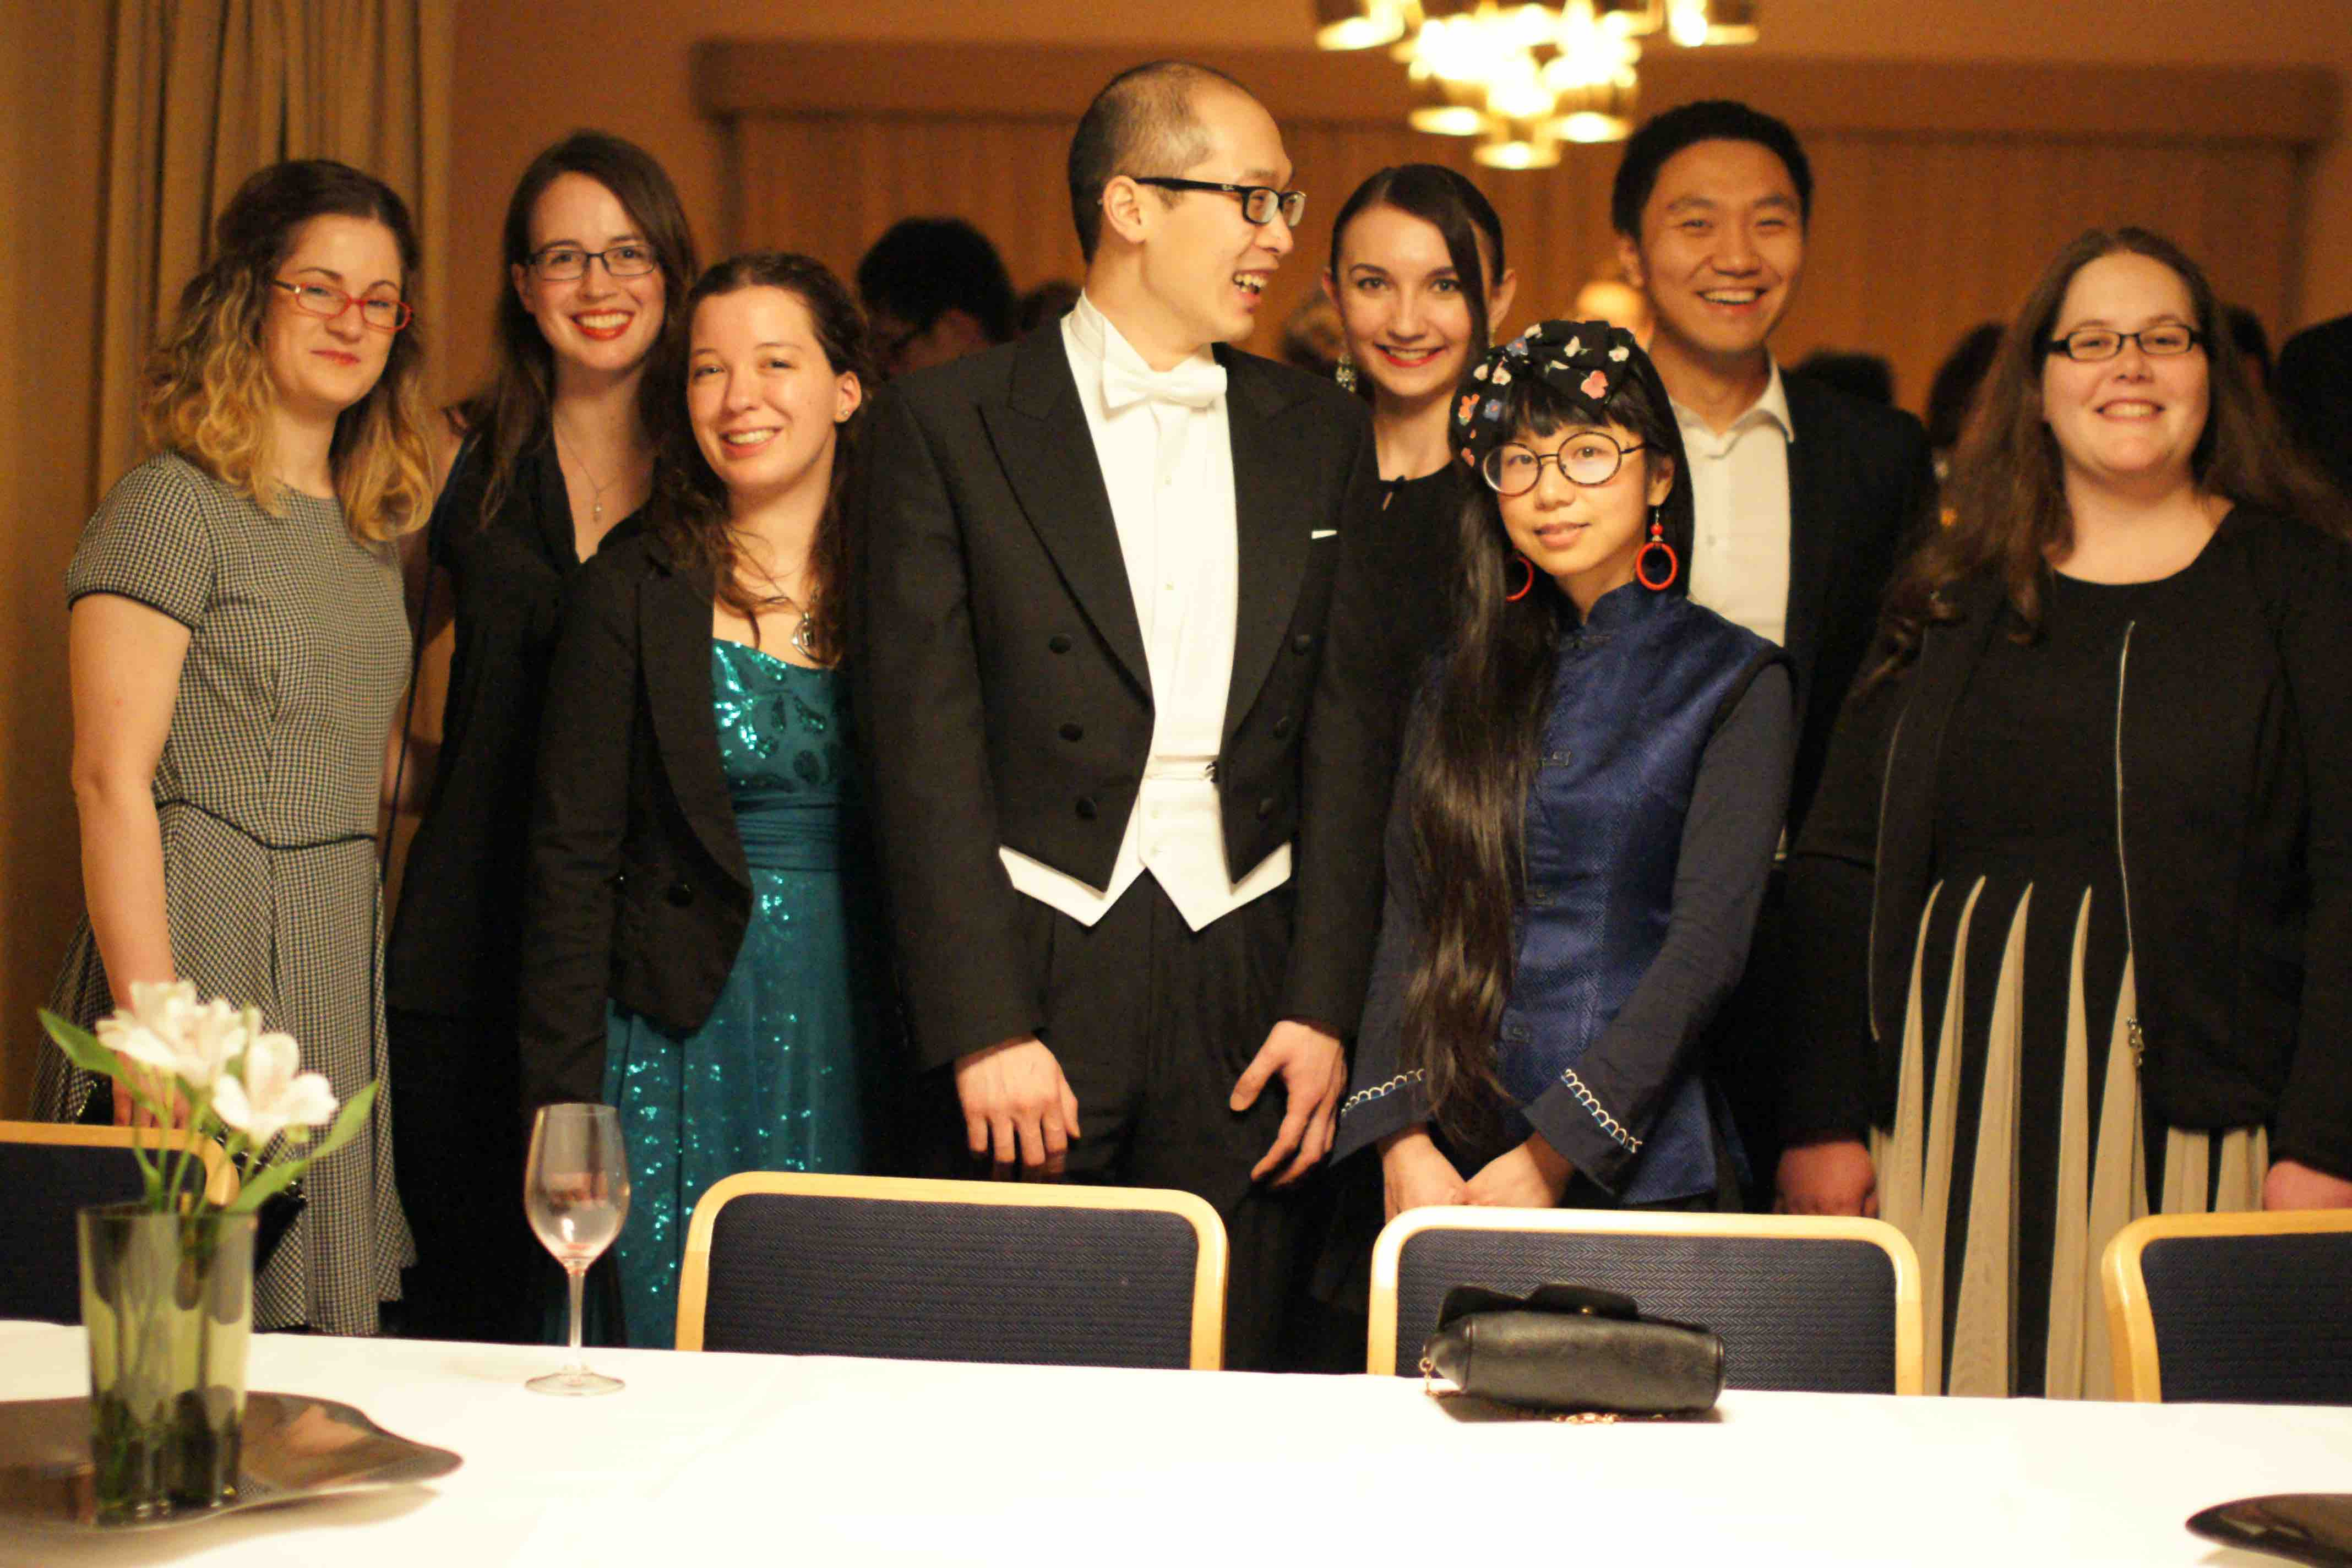
\includegraphics[scale=0.02,angle=0]{./plots/kk3.jpg}
		\end{center}
		\item Phd
		\begin{center}
			
\includegraphics[scale=0.02]{./plots/phd.jpg}
		\end{center}
	\end{itemize}
\end{frame}

\begin{frame}{Awards (name vs money)}
	\begin{itemize}
		\item Chinese government awards for outstanding Phd candidate
		\begin{center}
			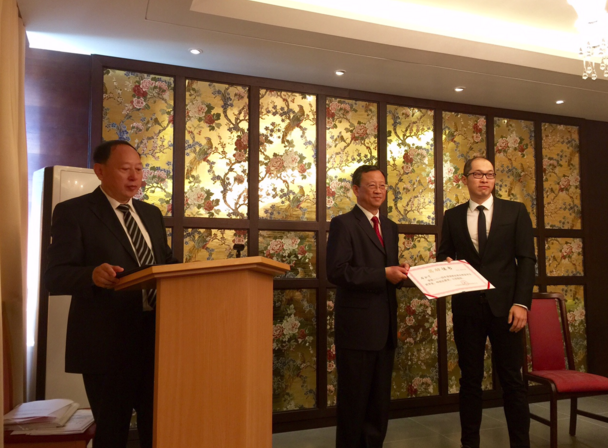
\includegraphics[scale=0.3]{./plots/awards1.png}
		\end{center}
		\item Some awards from Aalto university.
	\end{itemize}
\end{frame}

\begin{frame}{What did I learn from Phd?}
	\begin{itemize}
		\item Strong expertise in
		\begin{itemize}\footnotesize
			\item Machine learning and mathematical modelings
			\item Optimization research: linear/nonlinear optimizations
			\item Algorithm and data analysis / recommender system
			\item Large scale data analysis
		\end{itemize}
		\item Solid programming skills in
		\begin{itemize}\footnotesize
			\item Python, Matlab, C
			\item Hadoop, Spark, SQL
			\item SVN, Git, Jekyll, JavaScript
			\item Website and blog at {\bf www.hongyusu.com}
			\item GitHub at {\bf www.github.com/hongyusu}
		\end{itemize}
		\item A creative brain to solve challenging problems with modern technologies.
		\item An open mind that always wants to learn.
		\item {\bf Be able to work hard for the long-term goal}.
	\end{itemize}
\end{frame}

\iffalse
\begin{frame}{Sentiment analysis}
	A small web application which can be built in a few days.
	\begin{center}
		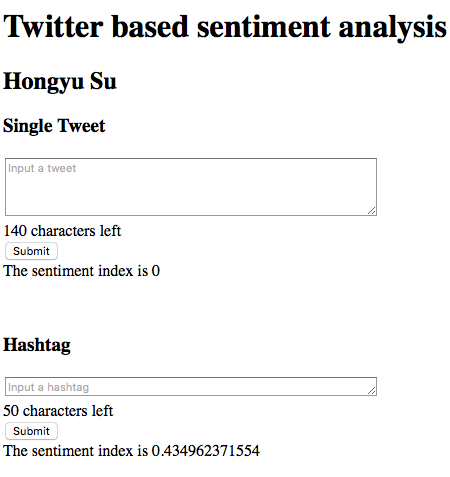
\includegraphics[scale=0.3]{./plots/norway.png}
		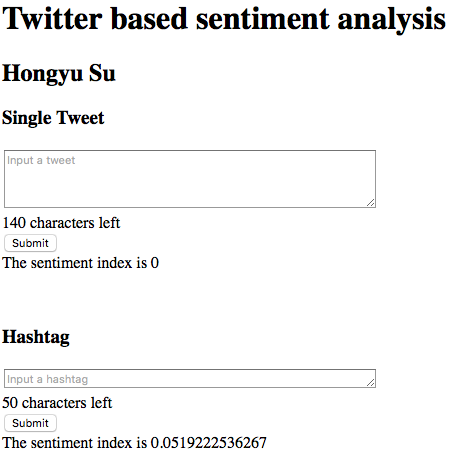
\includegraphics[scale=0.3]{./plots/finland.png}
	\end{center}
\end{frame}
\fi

\begin{frame}{A big fan of modern information technologies}
	\begin{itemize}
		\item I am curious, open, and want to learn new technologies.
		\item I am innovative, want to use new technologies to change daily life.
		\item Know new technologies very well, e.g., deep learning, big data, Kafka, Spark, IoT.
		\item Maintain a techical blog at {\bf www.hongyusu.com} on technology innovations.
		\item Double blade: new are not always good, e.g., I like old-fashion mechanical keyboard. 
	\end{itemize}	
	\begin{center}
		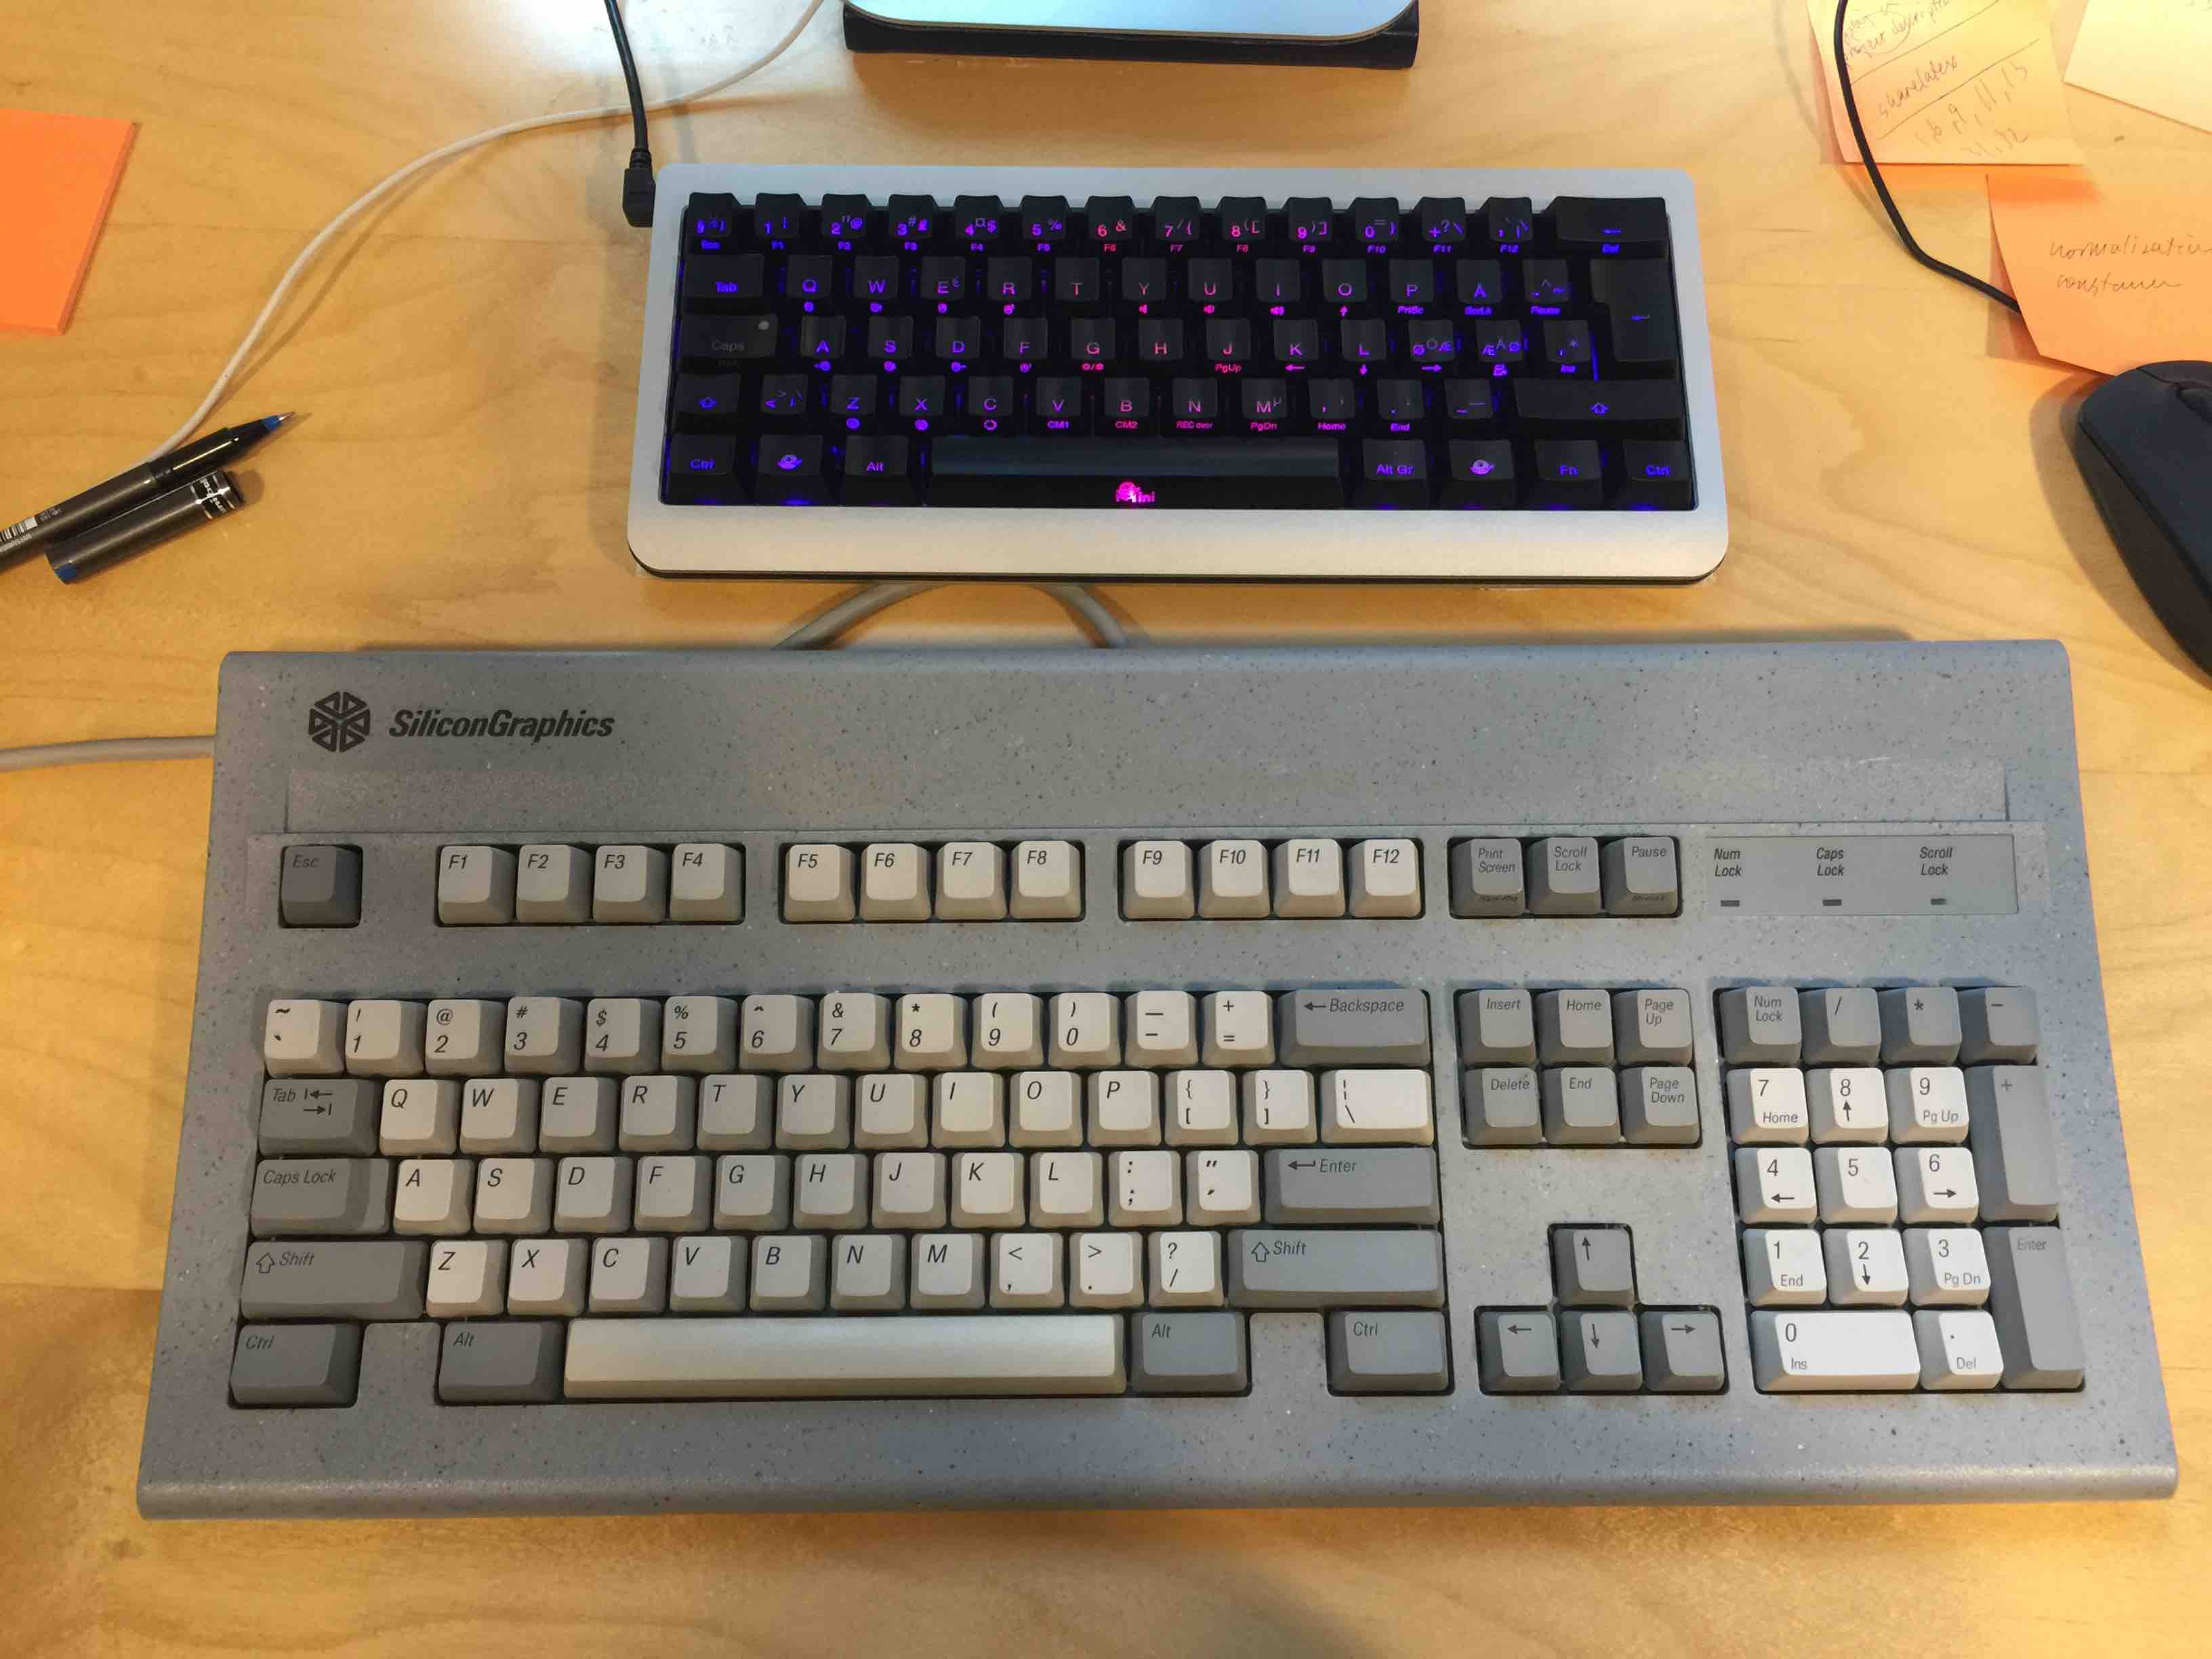
\includegraphics[scale=0.03]{./plots/keyboard.jpg}
	\end{center}
\end{frame}


\begin{frame}{A big fan of sports}
	\begin{itemize}
		\item I enjoy competitions and aggressive sport for example basketball.
		\begin{center}
			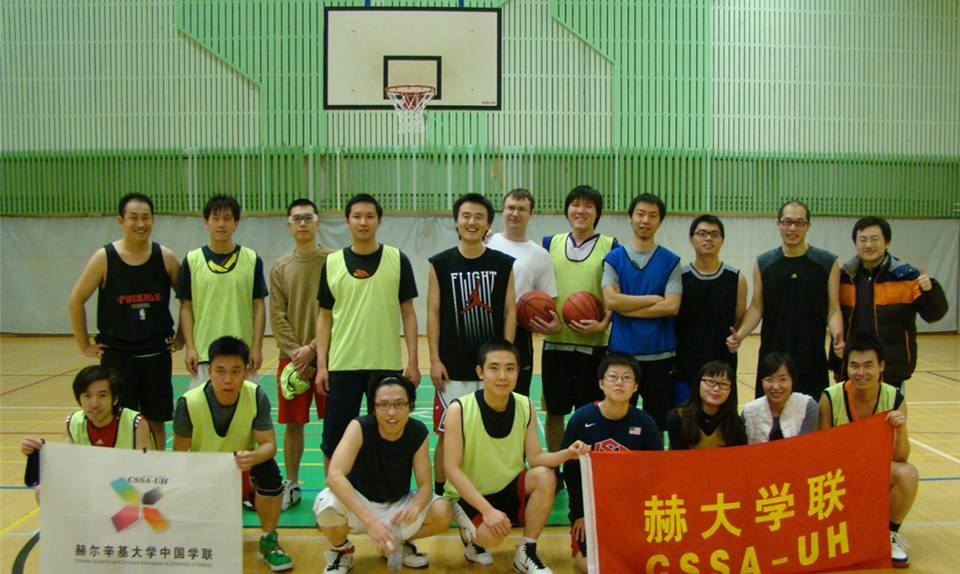
\includegraphics[scale=0.15]{./plots/basketball.jpg}
		\end{center}
		\item Now I try to discover unknown part of myself
		\begin{itemize}\footnotesize
			\item Downhill snowboarding.
			\item Bouldering (license)
			\item Paragliding 
			\item Open water diving (license)
		\end{itemize}
		\item A lot of gyms. 
	\end{itemize}
\end{frame}

\begin{frame}{A cat person}
	\begin{itemize}
		\item Pabulo
		\begin{center}
			%\includegraphics[scale=0.02,angle=-90,origin=c]{./plots/pabulo1.jpg}
			
\includegraphics[scale=0.15]{./plots/pabulo3.jpg}
		\end{center}
		\item Miu
		\begin{center}
			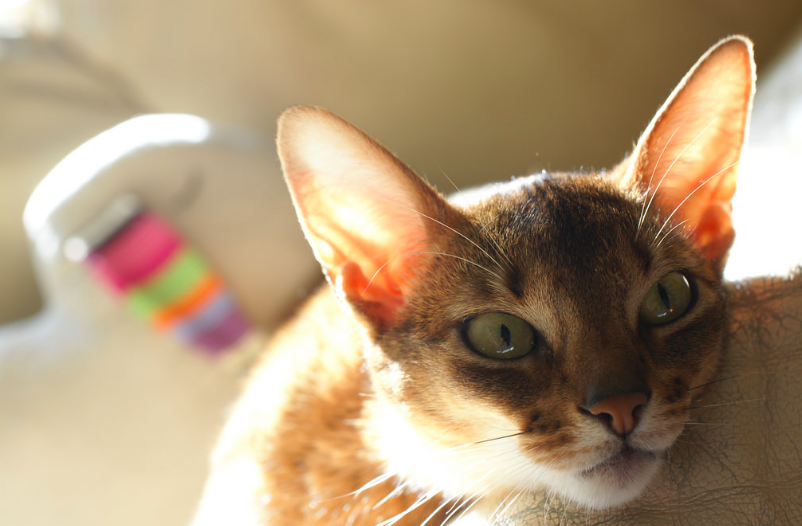
\includegraphics[scale=0.15,origin=c]{./plots/miu.jpg}
		\end{center}
		\item Cats are independent and make my life not very technical.
	\end{itemize}
\end{frame}


\begin{frame}{A hiker}
	I like to discover new places.
	\begin{center}
		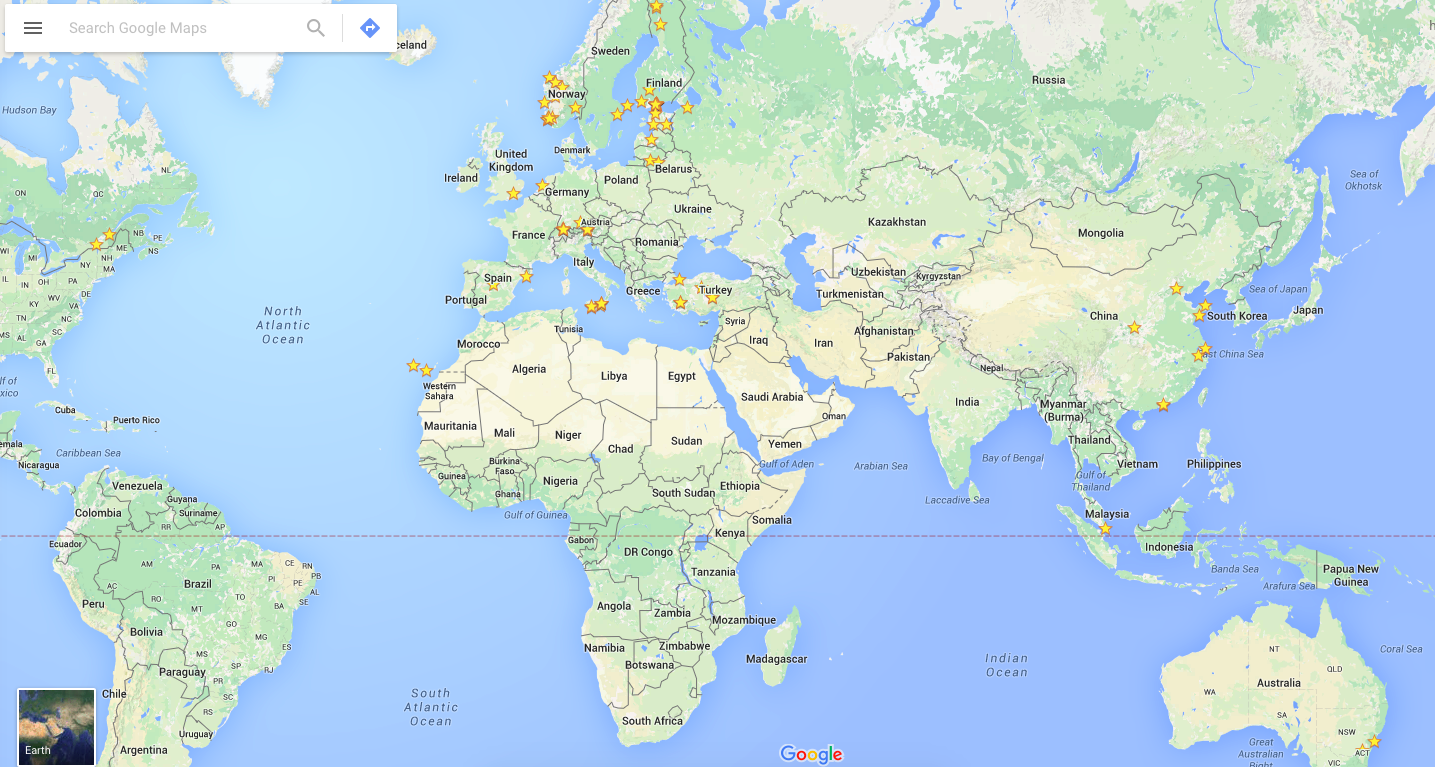
\includegraphics[scale=0.22,angle=-0,origin=c]{./plots/googlemap.png}
	\end{center}
\end{frame}

\begin{frame}{A photographer with a Flickr account}
	I like to memorize great moments.
	\begin{center}
		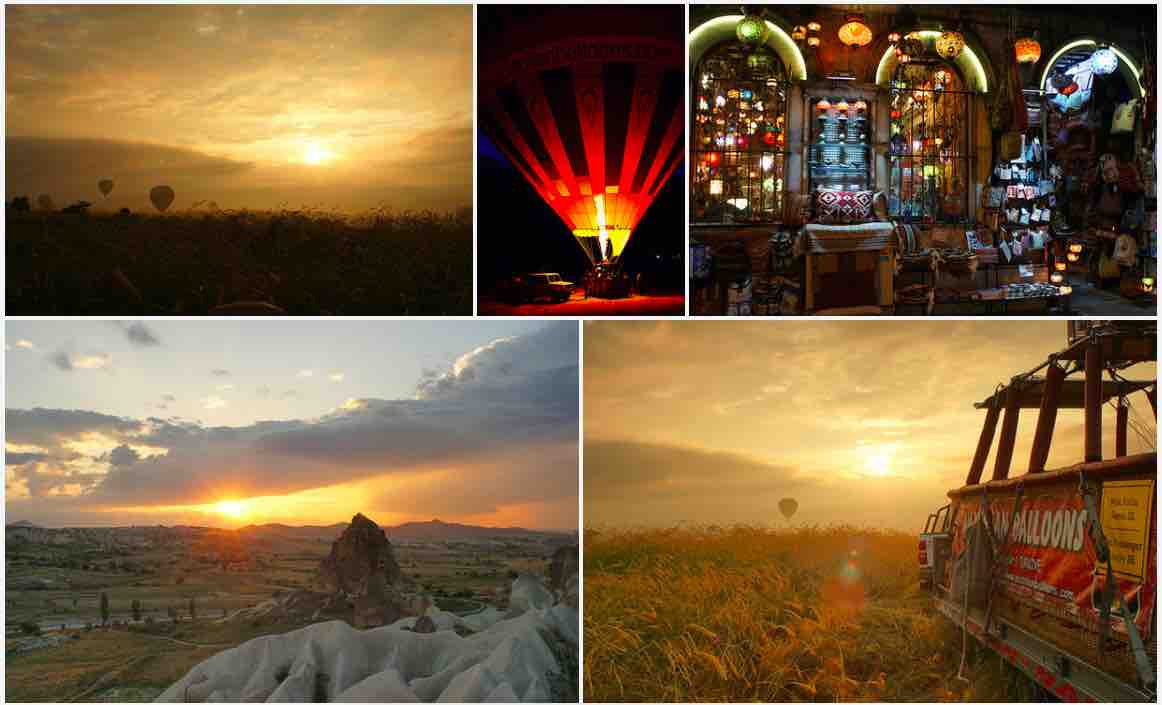
\includegraphics[scale=0.25,angle=-0,origin=c]{./plots/flickr.jpg}
	\end{center}
\end{frame}

\begin{frame}{A bottle collector}
	I like to taste new things.
	\begin{center}
		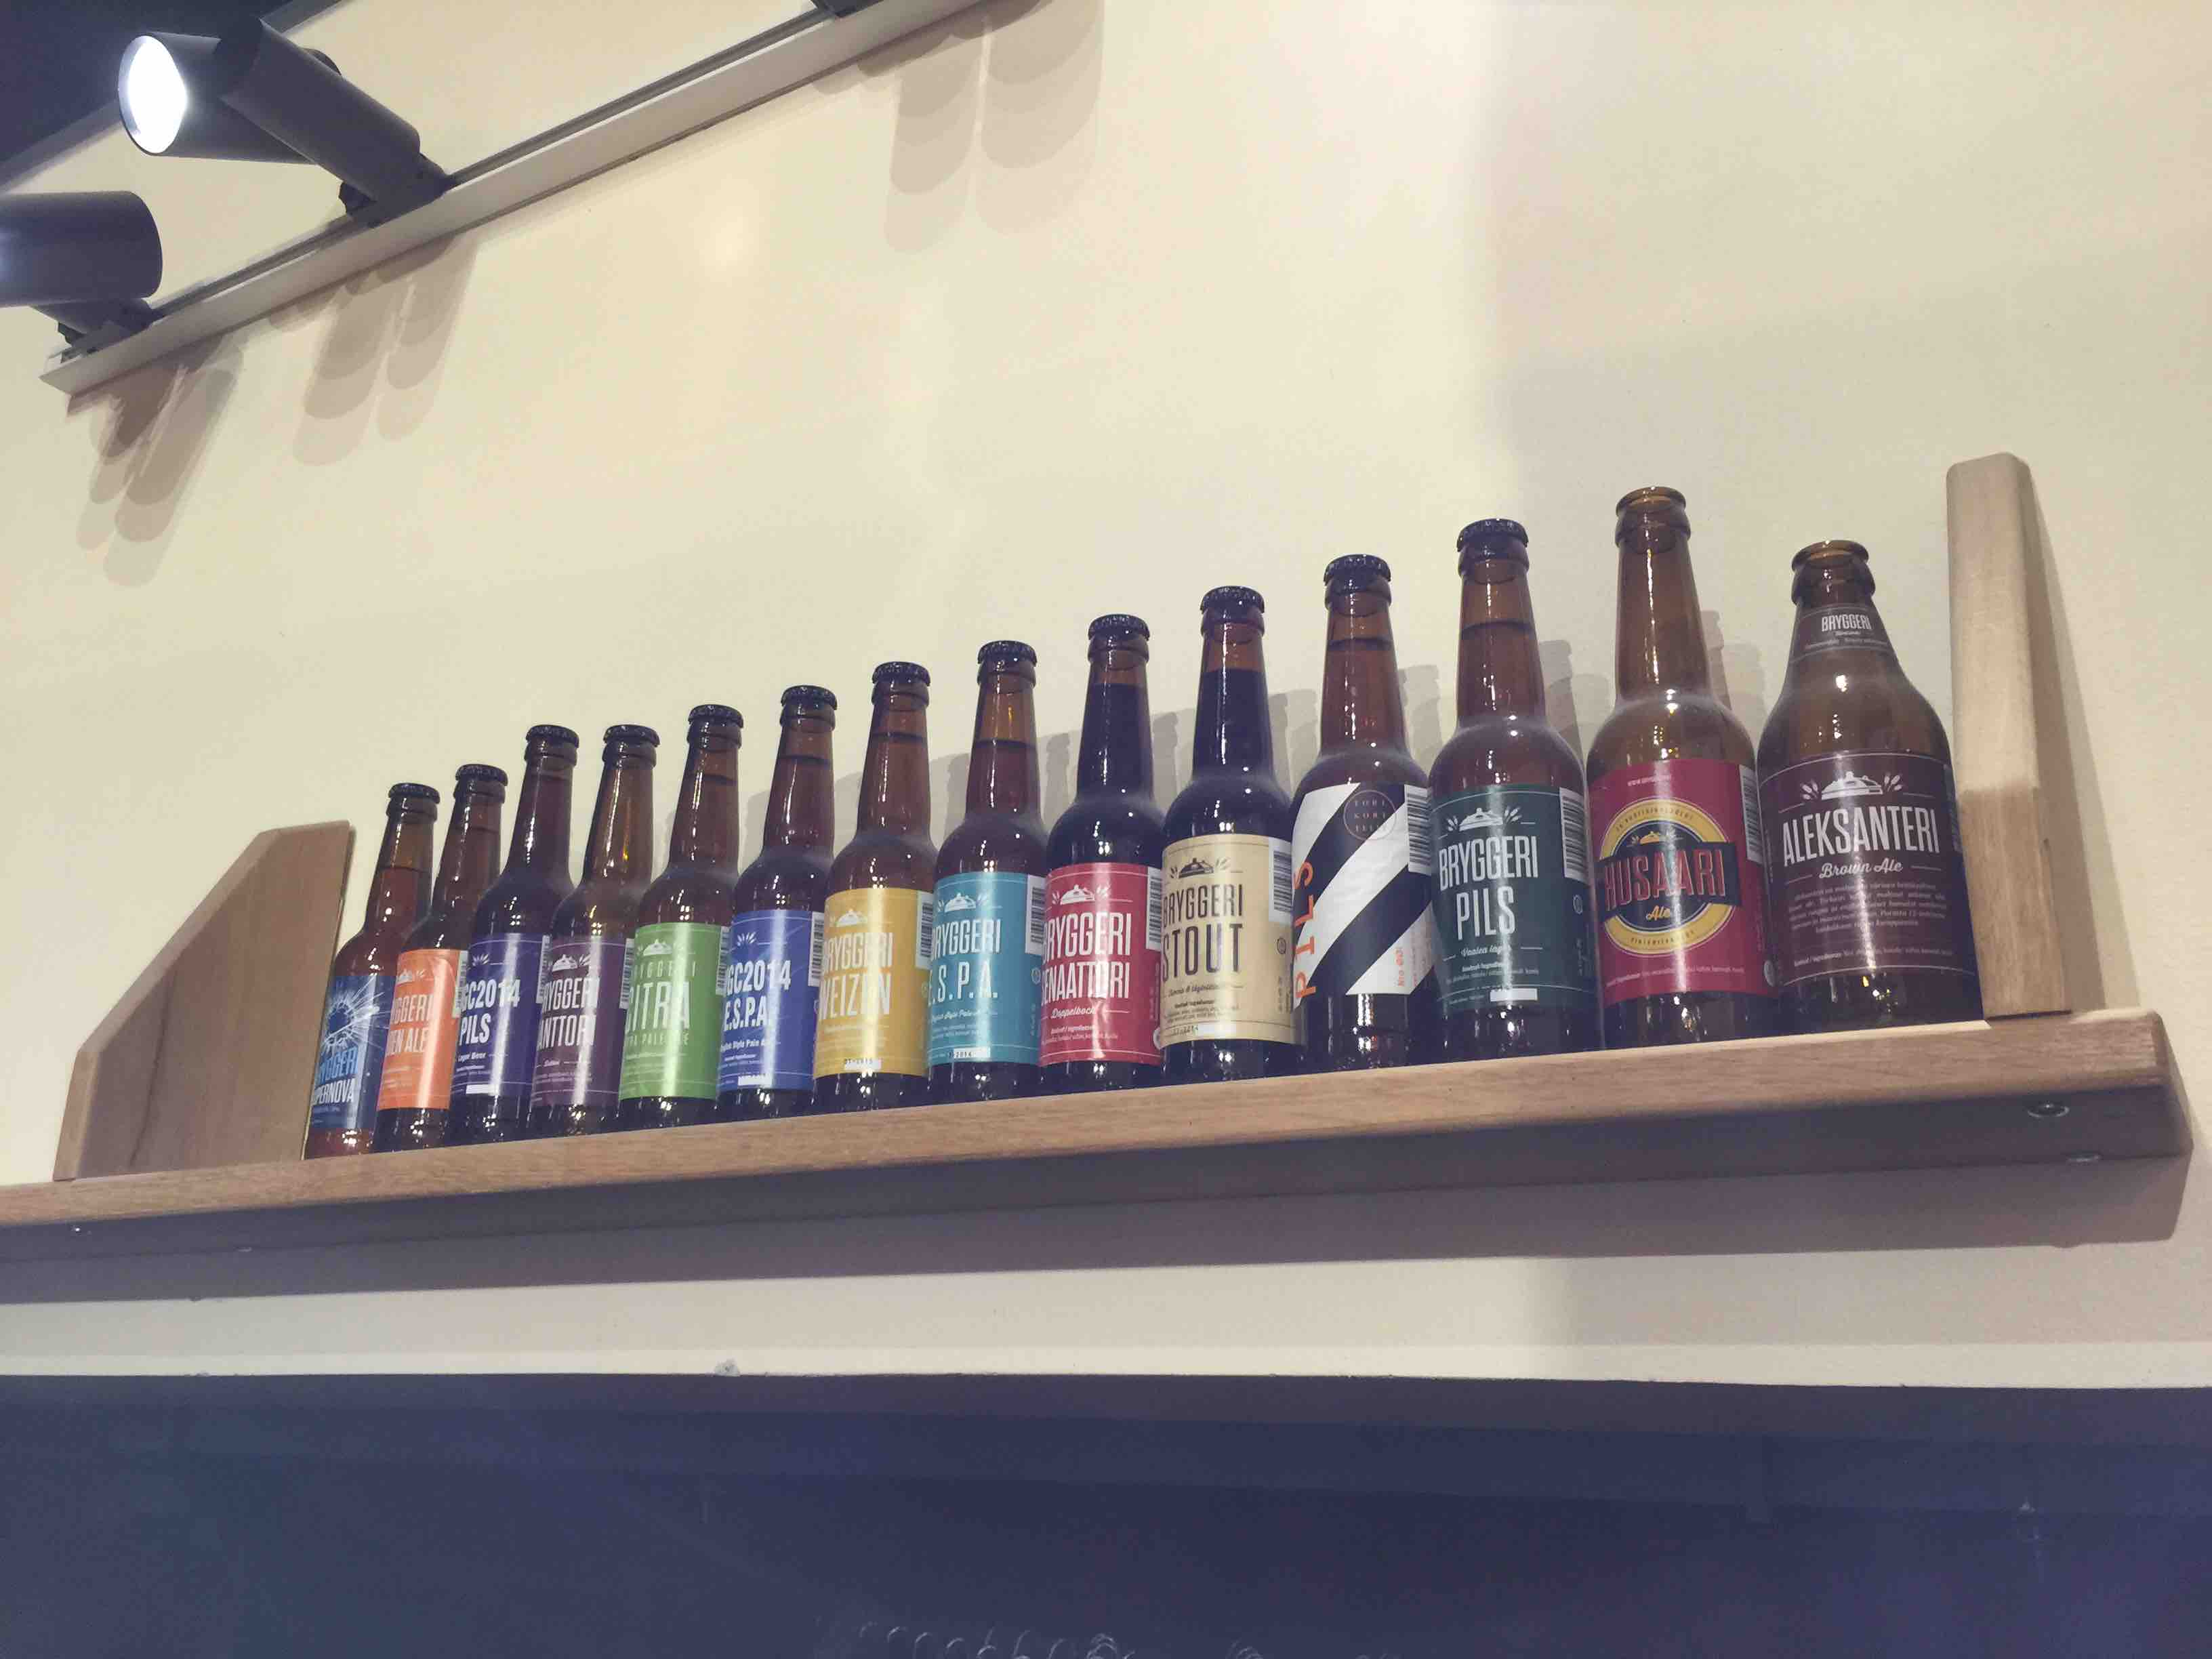
\includegraphics[scale=0.05,angle=-0,origin=c]{./plots/bottle1.jpg}
	\end{center}
\end{frame}

\begin{frame}{}
	\begin{center}
		{\em `Stay hungry, stay foolish.'} - Steve Jobs
	\end{center}
\end{frame}

\end{document}
